\chapter{Development of an optimisation framework for conceptual aircraft design}
\markboth{Development of an optimisation framework for conceptual aircraft design}{Development of an optimisation framework for conceptual aircraft design}
\label{chap2:fast_base_mdo}

%\begin{mdframed}[hidealllines=true,backgroundcolor=lightgray!20]
%	\section*{Résumé}
%	Ce chapitre présente l’élaboration d’un cadre pour le dimensionnement et l’optimisation d’un avion de grande capacité. 
%	Le code développé repose sur l'intégration de FAST dans la plate-forme d'optimisation multidisciplinaire OpenMDAO.
%	
%	FAST est un outil d'analyse de conception multidisciplinaire développé par l'ONERA et l'ISAE-Supaero pour le dimensionnement d'aéronefs conventionnels. 
%	Entièrement écrit en Python, il est basé sur les méthodes classiques du manuel de conception et sur une approche de masse ponctuelle pour l’estimation des performances. 
%	La boucle de dimensionnement regroupe toutes les disciplines clés de la conception des aéronefs: aérodynamique, structure/masse, propulsion, performances, ainsi que certains aspects liés aux spécifications de certification. 
%	Le scénario de test de validation de FAST est l’avion CERAS d’Airbus A320.
%	
%	OpenMDAO est plutôt une plate-forme d'optimisation multidisciplinaire développée par la NASA Glenn Research Center. 
%	Ce intègre une grande variété d'algorithmes d'optimisation, déjà inclus dans les bibliothèques Python, dans un code créé spécifiquement pour faciliter la définition de problèmes d'optimisation de conception multidisciplinaire. 
%	Grâce à sa logique, composée de modules indépendants, le problème peut être décomposé et organisé au plus haut niveau très facilement~: cette approche modulaire permet de remplacer certaines disciplines avec des modifications mineures. 
%	La principale caractéristique d'OpenMDAO est liée à MAUD, qui constitue un moyen innovant de calculer des dérivés pour résoudre des problèmes d'optimisation. 
%	Grâce à MAUD, OpenMDAO peut calculer efficacement les dérivées, en réduisant le coût de calcul, et il est principalement adapté aux optimisations basées sur les gradients. 
%	Son succès est attesté par la grande variété de travaux faisant appel à OpenMDAO que ce soit dans le cadre de problèmes aéronautiques et aérospatiaux ou d’autres sujets.
%	
%	Pour intégrer FAST dans OpenMDAO, le code doit être modifié et réorganisé: les anciennes disciplines sont décomposées en différents modules~; pour faciliter l'utilisation du gradient, chaque module correspond à une équation. 
%	À un niveau supérieur, les critères de conception, par exemple pour les surfaces d'aile et d’empennage, sont remplacés par la définition de contraintes de conception pour le problème d'optimisation, afin de permettre à l'optimiseur de trouver la meilleure solution dans l'espace de conception. 
%	Grâce aux méthodes numériques efficaces et à la logique d'OpenMDAO, le coût de calcul a été réduit de 5 minutes à environ 30 secondes pour une seule itération. 
%	Cependant, il présente l’inconvénient que la modularité a introduit 200 nouvelles fonctions, au lieu des 20 fonctions utilisés précedemment 20, ce qui peut compliquer la compréhension du code par un nouvel utilisateur.
%	La formulation résultante de l'optimisation multidisciplinaire est l’architecture MDF, qui apparaît comme la plus appropriée au problème de conception d'aéronef, bien qu'elle nécessite la définition d'une boucle complète d'analyse de conception multidisciplinaire.
%
%	La version intégrée a été appliquée sur le scénario du cas test CERAS: les résultats montrent que l'optimisation entraîne une réduction de la consommation de carburant d'environ 10\%, ce qui n'est pas négligeable en pourcentage.
%	Ensuite, l’avion CERAS est redimensionné en tenant compte de différentes plages de conception et d’hypothèses technologiques pour l’horizon 2035, afin d’obtenir un ensemble d’aéronefs de référence à utiliser pour la comparaison avec les configurations non conventionnelles qui seront proposées dans les chapitres suivants.
%	
%	Il est à mentionner que le travail d'intégration a été effectué en collaboration avec le MDO Lab. à l'Université du Michigan, lors d'une visite de 3 mois de janvier à avril 2018, avec le support financier de la Formaction Doctorale ISAE-Supaero.
%\end{mdframed}
%
%\cleardoublepage

\minitoc

\clearpage

\begin{mdframed}[hidealllines=true,backgroundcolor=purple!20]
	\section*{Outline}
	
	\begin{itemize}
	
		\item Description of FAST, the ONERA and ISAE-Supaero aircraft sizing tool, is given. 
		
		\item OpenMDAO, the multidisciplinary optimisation tool from NASA Glenn Research Centre, is presented. Notions on its logic are given, to understand the development of MDO problems. 
		
		\item An integrated sizing tool is obtained from the coding of FAST within the OpenMDAO platform. 
		
		\item The integrated code FAST and OpenMDAO is used to optimise the Airbus A320 CERAS test case. 
		
	\end{itemize}

\end{mdframed}

\cleardoublepage

\section{Introduction}
\label{sec:chap2_intro}

This chapter presents the sizing tool developed in this research to obtain a MDO procedure, considering the test case of a conventional aircraft. 
It comes from the integration of FAST~\cite{bib:fast_main}, an in-house code developed at ONERA and ISAE-Supaero, into OpenMDAO, an optimisation platform developed at NASA Langley Research Centre~\cite{bib:openmdao_website, bib:gray_omdao}. 

At first, Sec.~\ref{sec:chap2_fast_base_description} presents a description of the original code FAST, including discipline models and validation cases. 
Then, Sec.~\ref{sec:chap2_openmdao_overview} describes the multidisciplinary optimisation platform OpenMDAO, highlighting its capabilities and main features for optimisation problems.
Finally, the integration of FAST into OpenMDAO is reported in Sec.~\ref{sec:chap2_fast_omdao_base}, where the recoding work is detailed. 
This section gives also the chance to highlight differences between the MDA and the MDO approach, showing that the latest is more accurate when dealing with a large number of disciplines, thanks to the way the design constraints are defined. 
The new framework is then evaluated on the Airbus A320 CERAS test case~\cite{bib:ceras}, to assess the optimisation process, and is then used to define the reference aircraft, to compare with the hybrid and the BWB concept later. 

It must be mentioned that the work described in this chapter has been done in collaboration with the MDO Lab., at University of Michigan, during a visit conducted from January to April 2018.
The visit has been funded thanks to a grant for international exchange from \textit{Formation Doctorale} of ISAE-Supaero. 

\section{The sizing tool FAST}
\label{sec:chap2_fast_base_description}

\subsection{Overview}
\label{subsec:chap2_fast_overview}
FAST (Fixed-wing Aircraft Sizing Tool) is an in-house software, developed by ONERA and ISAE-Supaero, for aircraft sizing and analysis purposes~\cite{bib:fast_main}. 
Fully developed in Python 2.7, in its native version, it is a multidisciplinary code, capable to carry out the preliminary sizing of a turbofan aircraft, for given top level requirements (TLAR), and evaluate its performance.
The validation case is the A320 CERAS test case~\cite{bib:schmollgruber}, based on the Airbus A320 data~\cite{bib:a320_specifications}. 
During the process, it considers all the key disciplines in aircraft design: aerodynamics, structure/mass estimation and propulsion. 
Since FAST is tailored for the conceptual design, models are based mainly on semi-empirical equations, coming from classical design handbooks~\cite{bib:roskam_partI, bib:raymer} and Airbus experience and collected in the ISAE-Supaero notes~\cite{bib:airbus_notes}, which are accurate as long the conventional TAW configuration is considered. 

FAST interfaces also with other softwares, that are used for aerodynamics computation: XFOIL~\cite{bib:xfoil} for airfoil performance and OpenVSP~\cite{bib:openvsp} for the low speed polars. 
The last one is also used for visualisation purposes at the end of the sizing procedure. 
An \texttt{xml} file (eXtensible Markup Language) is used for the flow data: it containts the initial set of TLAR and collects the output variables of the design process. 
Thus the \texttt{xml} file is the I/O file for the FAST workflow.

After its first developments, FAST has been successfully used in several projects, and it is now been expanded to consider regional aircraft, ATR type~\cite{bib:bohari}, and to interface with a certification constraint module and full mission simulations~\cite{bib:schmollgruber, bib:schmollgruber_phd}. 
The next sections give an outlook to the main elements of FAST: Sec.~\ref{subsec:chap2_fast_xml_struc} describes I/O file structure, Sec.~\ref{subsec:chap2_fast_mod_desc} reports details of  a description of all the parts of the software, and Sec.~\ref{subsec:chap2_fast_test_case} reports the results for the validation test case.  

\subsection{I/O structure file}
\label{subsec:chap2_fast_xml_struc}

To manage the dataflow, FAST relies on an \texttt{xml} file. 
This format is mainly indicated for the management of a large data flow, since it facilitates the inputs and the outputs, and is well interfaced with Python, thanks to the dedicated libraries~\cite{bib:nagel_cpacs}. 

FAST uses GAMME for reading and writing~\cite{bib:bedouet}: it is a meta-model, capable to automatically create Python dictionaries from the \texttt{xml} file. 
It can also handle units and their conversion, which is an added feature of relevance in aircraft design, where input data can be given following different unit systems.

The main argument of \texttt{xml} file is called \texttt{Aircraft}. 
Then this argument is structured in nine subparts, on different levels (from input data to output per discipline), as follows:
\begin{itemize}
	\item \textbf{TLAR.} This section contains the top level requirements for the aircraft: aircraft type (large passenger, business jet, \textellipsis), range, number of passengers, approach speed, cruise Mach number and maximum allowable takeoff runway length.
	
	\item \textbf{Configuration.} This section contains the parameters used to define the configuration, such as engine location or empennage type. Each of these specifications is identified by a numerical flag.
	
	\item \textbf{Mission.} This section contains the parameters to define the given mission, and, as outputs, the relative fuel breakdown, time of flight and takeoff/landing performances.
	This section has two sublevels: one related to the design mission, and another one to operational missions.
	
	\item \textbf{Cabin.} This section is used to define all the parameters for the internal cabin layout.
	
	\item \textbf{Geometry.} This section is dedicated to the geometry. 
	It is divided into several sublevels, one for each geometrical component: in each sublevel there are a few sets of inputs.
	As outputs, all the geometrical dimensions are reported. 
	This section is also shared with the OpenVSP visualisation tool, in order to create a 3D sketch of the aircraft at the end of the sizing loop.
	
	\item \textbf{Propulsion.} This section contains the input parameters for the engine definition, according to the chosen model, as it will be described later. 
	
	\item \textbf{Aerodynamics.} This section is solely for output, and it stores global aerodynamics parameters.
	
	\item \textbf{Weight.} This section is for the mass breakdown, and it is divided into sublevels: airframe, propulsion, secondary systems, furniture and crew. 
	The breakdown is made according to the standard defined by the French norm AR 2001/D~\cite{bib:mass_breakdown}.
	
	\item \textbf{Balance.} This section shows the same structure as the \texttt{Weight} section, but instead of masses it contains all the center of gravities positions, plus the global center of gravity. 
	It is also used to define the maximum allowable CG range variation, used to satisfy stability requirements.
\end{itemize}
An example of \texttt{xml} file structure is reported in Appendix~\ref{app:xml_file_struct}.

Accessing a file is a costly procedure in programming, even with dedicated libraries that facilitates the reading and writing: for this reason, FAST reads the \texttt{xml} file one time at the beginning of the process, to store all the input variables.
Afterwars, it accesses to the file again at the end of sizing, for output writing purposes. 

Finally, it must be highlighted that \texttt{xml} format has been largely used in aircraft design: a standard, called CPACS, is defined as common language, to facilitate the data sharing~\cite{bib:nagel_cpacs}. 
To enlarge the possible utilisation of the software, FAST is provided with a CPACS converter, to switch between this standard and the native \texttt{xml} standard for FAST. 

\subsection{Code description}
\label{subsec:chap2_fast_mod_desc}

The code is described in Fig.~\ref{fig:fast_basic}, with the xDSM standard, meanwhile the detailed algorithm (with the numbering referred to the figure) is reported below in Alg.~\ref{alg:fast_basic}. 
The scheme shown in Fig.~\ref{fig:fast_basic} highlights the multidisciplinary nature of the software: disciplines are connected each others and exchange lot of data, as indicated by the grey line. 
\begin{figure}[!h]
	\centering
	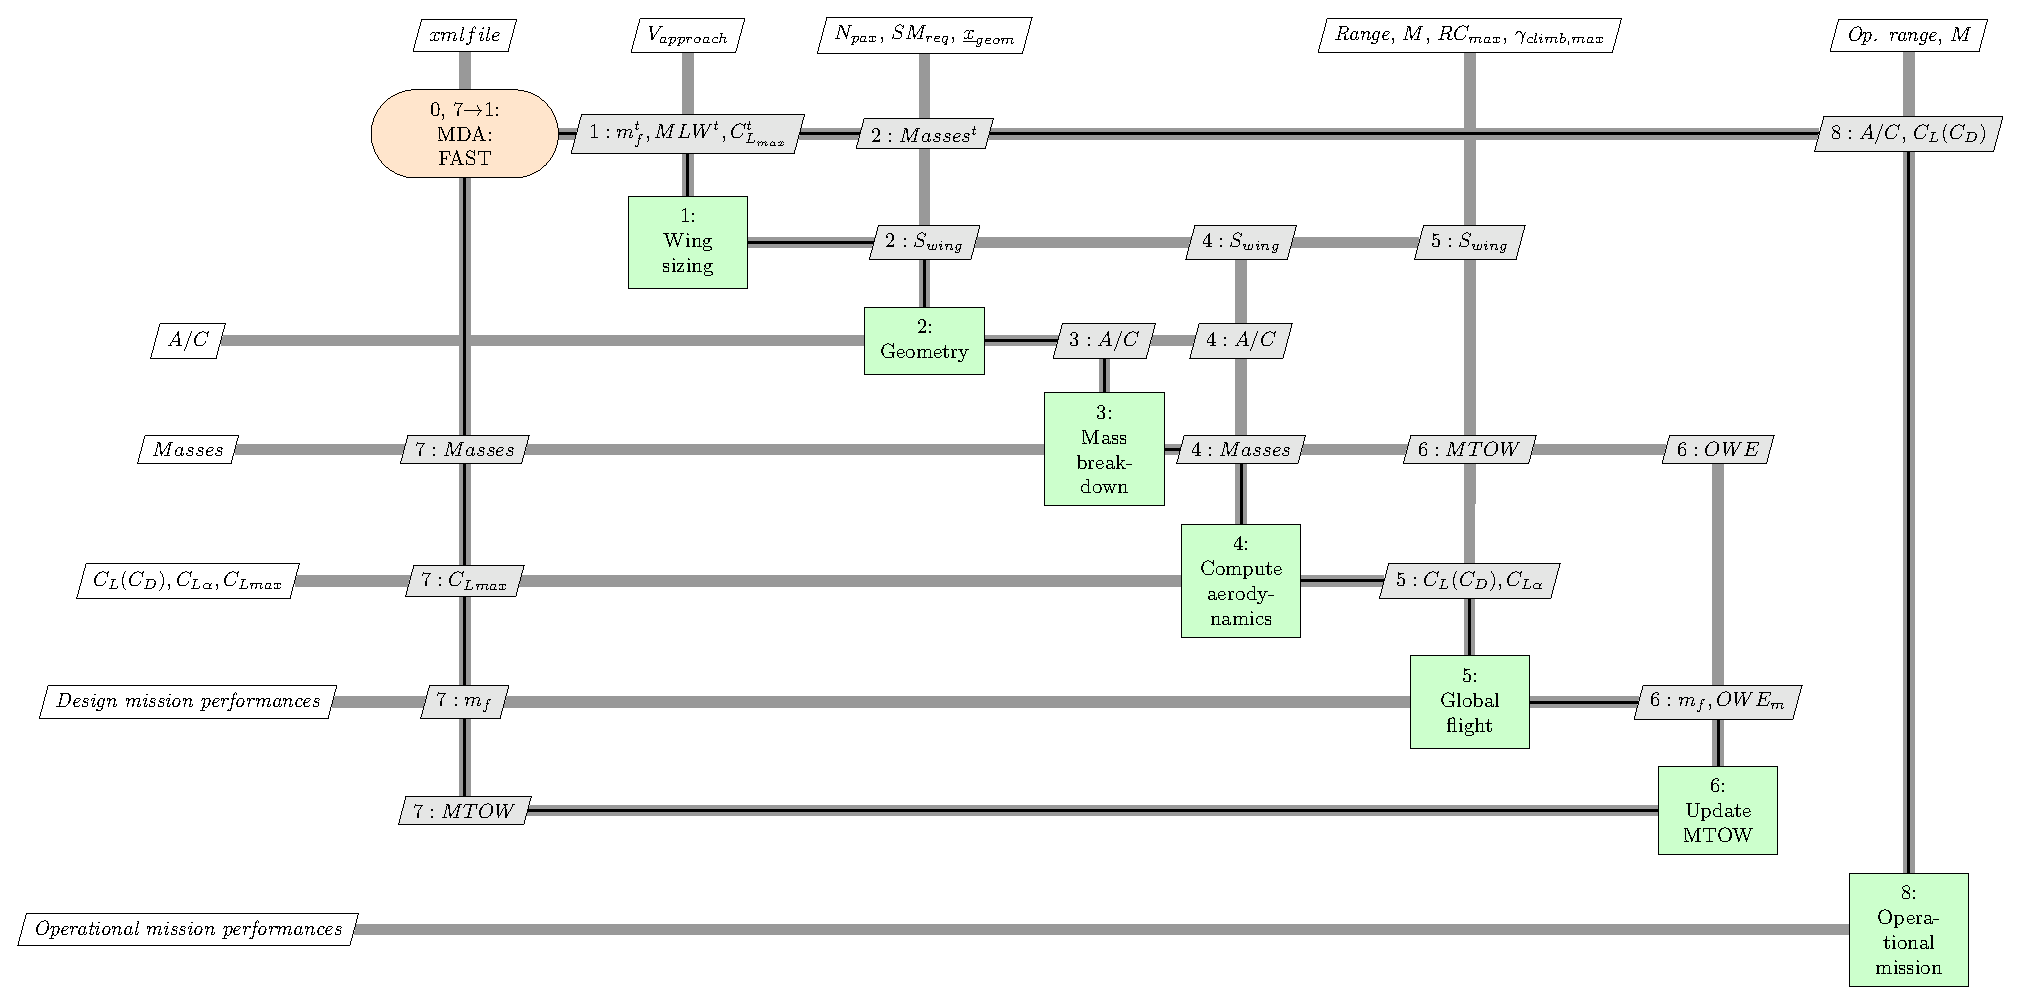
\includegraphics[keepaspectratio, width=1.2\textwidth, angle=90]{images/chap2/FAST}
	\caption{Diagram of FAST, using the xDSM standard~\cite{bib:lambe_xdsm}.}
	\label{fig:fast_basic}
\end{figure}

\begin{algorithm}[!h]
	\caption{FAST algorithm. Numbering is referred to diagram shown in Fig.~\ref{fig:fast_basic}.}
	\label{alg:fast_basic}
	\begin{algorithmic}
		\REQUIRE Initial design parameters (TLAR)
		\ENSURE Sized aircraft, drag polars, masses, design mission trajectory
		\STATE 0: Initialise the loop with a first estimate of geometry and masses, with the values from the \texttt{xml} file~\cite{bib:airbus_notes}. At this step engine is initialised too.
		\REPEAT
		\STATE 1: The wing area is obtained in order to supply enough lift in landing condition and to store all the fuel needed for the design mission.
		\STATE 2: The aircraft geometry is deduced through a resizing loop, to match the stability requirements.
		\STATE 3: Using the data coming from analysis 2, the masses and the center of gravities of each component are computed. Standard is the French norm AR 2001/D~\cite{bib:mass_breakdown}.
		\STATE 4: Aerodynamics analysis is carried out, to get the polars at low and high speed.
		\STATE 5: Performance calculation: the trajectory is performed through the integration of the flight equations using the Euler time step approach.
		\STATE 6: Update the value of MTOW, with the data coming from analyses 3 and 5.
		\STATE 7: Check the convergence: if the tolerance is below the needed threshold, return the sized aircraft, otherwise proceed to next iteration.
		\UNTIL {$7 \rightarrow 1$: MDA has converged}
		\STATE 8: Optionally, perform an operational mission, to assess the performance on different missions than the design one.
	\end{algorithmic}
\end{algorithm}

It must be noted that the engine is initialised outside the sizing loop, using the inputs from the \texttt{xml} file. 
The curves of thrust and specific fuel consumption SFC are obtained and provided to the performance analysis: in other words, FAST does not include the engine sizing in the design process.
Instead, it relies on a pre-existing engine deck, as will be detailed in Sec.~\ref{subsubsec:chap2_fast_propulsion}. 

The driven parameter for the MDA convergence is the operating weight empty OWE estimation.
There are two estimations for this parameter; the first one is obtained at analysis 3 as sum of all the airframe, propulsion, systems and furniture masses:
\begin{equation}
\label{eq:owe_struct}
m_{e_{3}} = \sum_{i=1}^{n}m_i
\end{equation}
where $i$ represents the generic component, as in the mass standard~\cite{bib:mass_breakdown}.

The second estimation is instead provided after the performance analysis:
\begin{equation}
\label{eq:owe_perf}
m_{e_{5}} = m_{TO} - m_f - m_{PL} 
\end{equation}

At convergence, the two values from Eq.~\eqref{eq:owe_struct} and Eq.~\eqref{eq:owe_perf} must be the same. 
The convergence criterion is then that the relative difference between the two does not exceed 0.05\%:
\begin{equation}
\label{eq:fast_conv_crit}
\left\lvert \frac{m_{e_{3}} - m_{e_{5}}}{m_{e_{3}}}\right\rvert \leq 5\times10^{-4}
\end{equation}
In case the error is above the value, MTOW is updated adding the difference between $m_{e_{3}}$ and $m_{e_{5}}$:
\begin{equation}
\label{eq:mtow_new}
m_{{TO}_{i+1}} = m_{{TO}_{i}} + \left(m_{e_{3}} - m_{e_{5}}\right)
\end{equation}

In next sections more details on the disciplinary analyses are provided. 
Indeed since they represent the starting point for the development aimed in this research, have a clear understanding of the models and their limit of validity is a key point.

\subsubsection{Propulsion}
\label{subsubsec:chap2_fast_propulsion}

In FAST the engine sizing is not included into the iterative process, but the curves representing its performances are provided to the code for the trajectory analysis. 
There are two engine's models that can be used in FAST: the first one is the engine deck used for the CERAS reference aircraft~\cite{bib:ceras}, meanwhile the second one is the so called ``rubber engine''~\cite{bib:roux}, which represents a model for the engine sizing, based on entries as thrust at sea level or BPR.

The CERAS engine is based on the deck used for the CERAS reference aircraft~\cite{bib:ceras}. 
The data are as close as possible to the Airbus A320's engine.
In particular, the by-pass ratio BPR is equal to 6 and the thrust at sea level is 117.8~\si{\kilo\newton}.  
The maps for thrust and fuel flow, as function of altitude and Mach, are provided to the performance module in FAST: according to the actual trajectory point, these parameters are evaluated through an interpolation. 
The maps are shown in Fig.~\ref{fig:ceras_engine_deck}.
The main limitation of this model is that thrust and fuel flow (then specific fuel consumption SFC too) are already provided, and there is no possibility to change the engine's parameters to obtain new curves. 
The field of application has been enlarged thanks to the definition of some corrective factors, that can be used to calibrate thrust and SFC; on top, this approach does not give any indication on the geometry data, so the impact on aerodynamics is neglected.
For a more detailed assessment a new model, that takes as input a set of engine parameters, must be defined.
\begin{figure}[!h]
	\centering
	\begin{subfigure}{0.45\textwidth}
		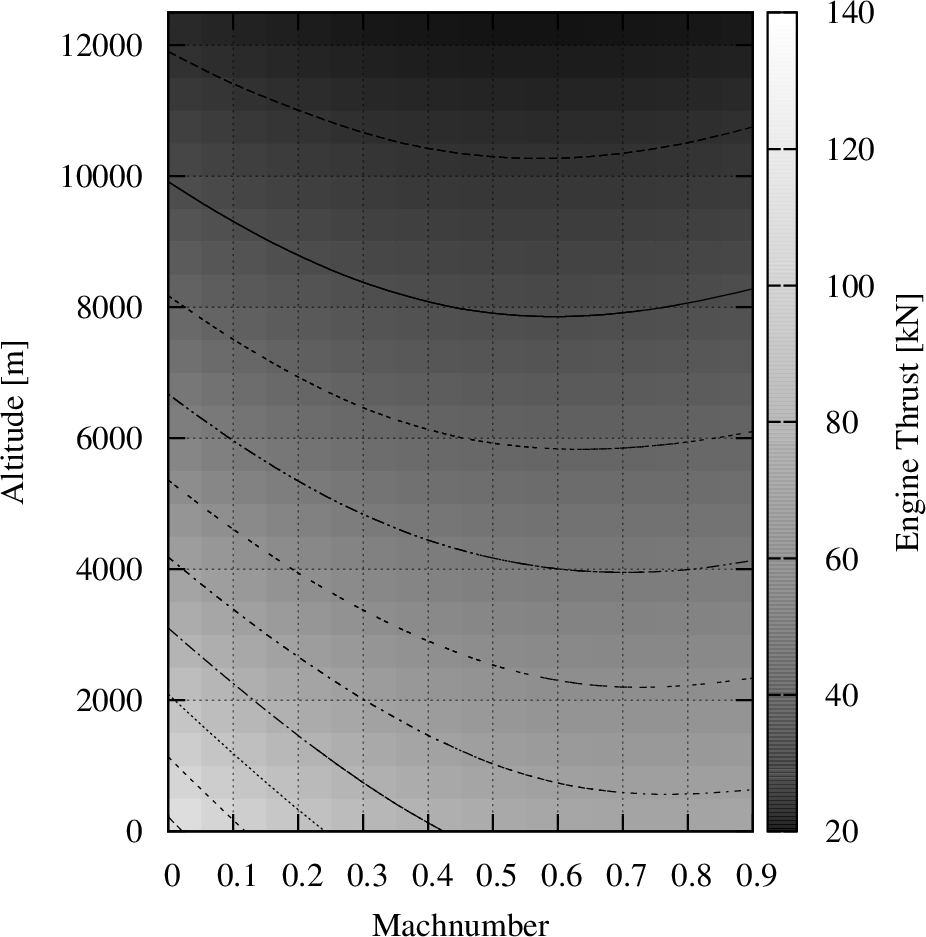
\includegraphics[keepaspectratio, width=\textwidth]{images/chap2/deck_thrust.png}
		\caption{Thrust data.}
		\label{subfig:ceras_thrust}	
	\end{subfigure}
	\begin{subfigure}{0.45\textwidth}
		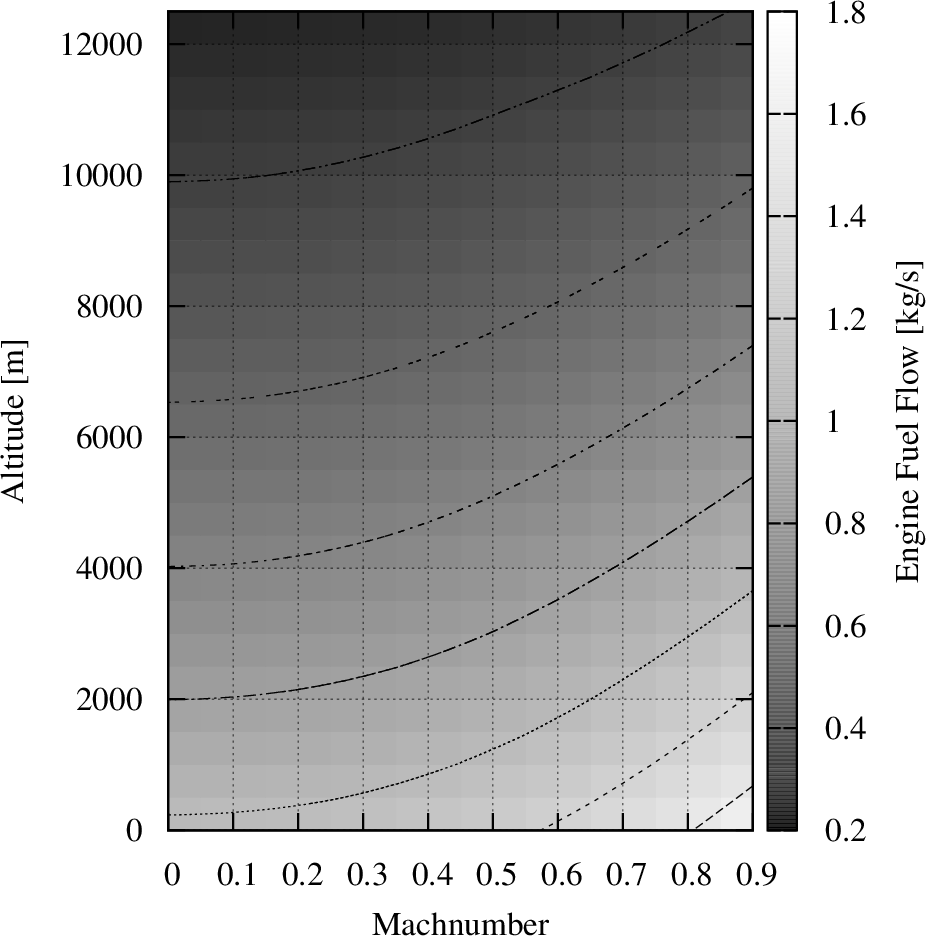
\includegraphics[keepaspectratio, width=\textwidth]{images/chap2/deck_ff.png}
		\caption{Fuel flow data.}
		\label{subfig:ceras_ff}	
	\end{subfigure}
	\caption{CERAS engine reference deck~\cite{bib:ceras}.}
	\label{fig:ceras_engine_deck}
\end{figure}

To this end, the ``rubber engine'' model has been developed by Roux in her Ph.D. thesis~\cite{bib:roux}: she based her equations on the previous formulations of Mattingly~\cite{bib:mattingly}, Jane Taylor~\cite{bib:janes}, Torenbeek~\cite{bib:torenbeek} and ESDU database~\cite{bib:esdu}. 
This model fixes the limitations of the CERAS deck, providing a set of equations to create the thrust and fuel flow maps, starting from a set of parameters: BPR, thrust at sea level, operating pressure ratio and temperature at the exit of the nozzle. 
It also provides the dimensions, giving an estimation of the engine wetted area, to consider also the impact on the aerodynamics.

\subsubsection{Geometry}
\label{subsubsec:chap2_fast_geom}

The geometry module is one of the key analyses to carry out, as it allows the definition of a viable aircraft, that satisfies OAD requirements, including balance and stability. 

Each aircraft component requires a set of input parameters from which it is possible to get geometrical properties and mass estimation. 
The choice of the entry parameters is not unique, but depends on the formulation; in FAST theoretical and statistical equations are applied, following the handbook provided by Airbus~\cite{bib:airbus_notes}.
Table~\ref{tab:fast_geom_entry_parameter} reports the set of parameters needed for each component; note that the wing needs the wing area, which is separately computed at step 2 of Fig.~\ref{fig:fast_basic}.  
Entries do not cover all the parameters needed: the remaining ones are computed starting from statistical equations that give the dependency with these entries.
As example, the thickness-to-chord ratio of the wing is computed considering the cruise Mach number, to take into account that it can not be too large to avoid compressibility at high speed~\cite{bib:airbus_notes}; in other formulations this parameter may be considered as input too. 
The same logic applied for the tails' aspect ratio and sweep. 
This aspect will become a key point in the development of the MDO problem, as it will be shown later.
\begin{table}[!h]
	\centering
	\begin{tabular}{c c c c}
		\hline
		\textbf{Fuselage} & \textbf{Wing} & \textbf{Tails} & \textbf{Engine and nacelle} \\
		\hline
		Number of passengers & Wing area & Taper ratio & Thrust at sea level \\
		Seats' dimensions & Aspect ratio & Thickness-to-chord ratio & Bypass ratio \\
		& Sweep angle & & \\
		& Taper ratio & & \\ 
		& Mach number & & \\
		\hline
	\end{tabular}
	\caption{Input parameters to properly size each geometrical component, according to the formulation used in FAST~\cite{bib:airbus_notes}.}
	\label{tab:fast_geom_entry_parameter}
\end{table}

The geometry analysis is an iterative procedure, that needs to converge, and thus it can be expressed with the usual xDSM diagram, as done in Fig.~\ref{fig:fast_geom_basic}. 
Corresponding algorithm is reported in Algorithm~\ref{alg:fast_geometry_basic}.
\begin{figure}[!h]
	\centering
	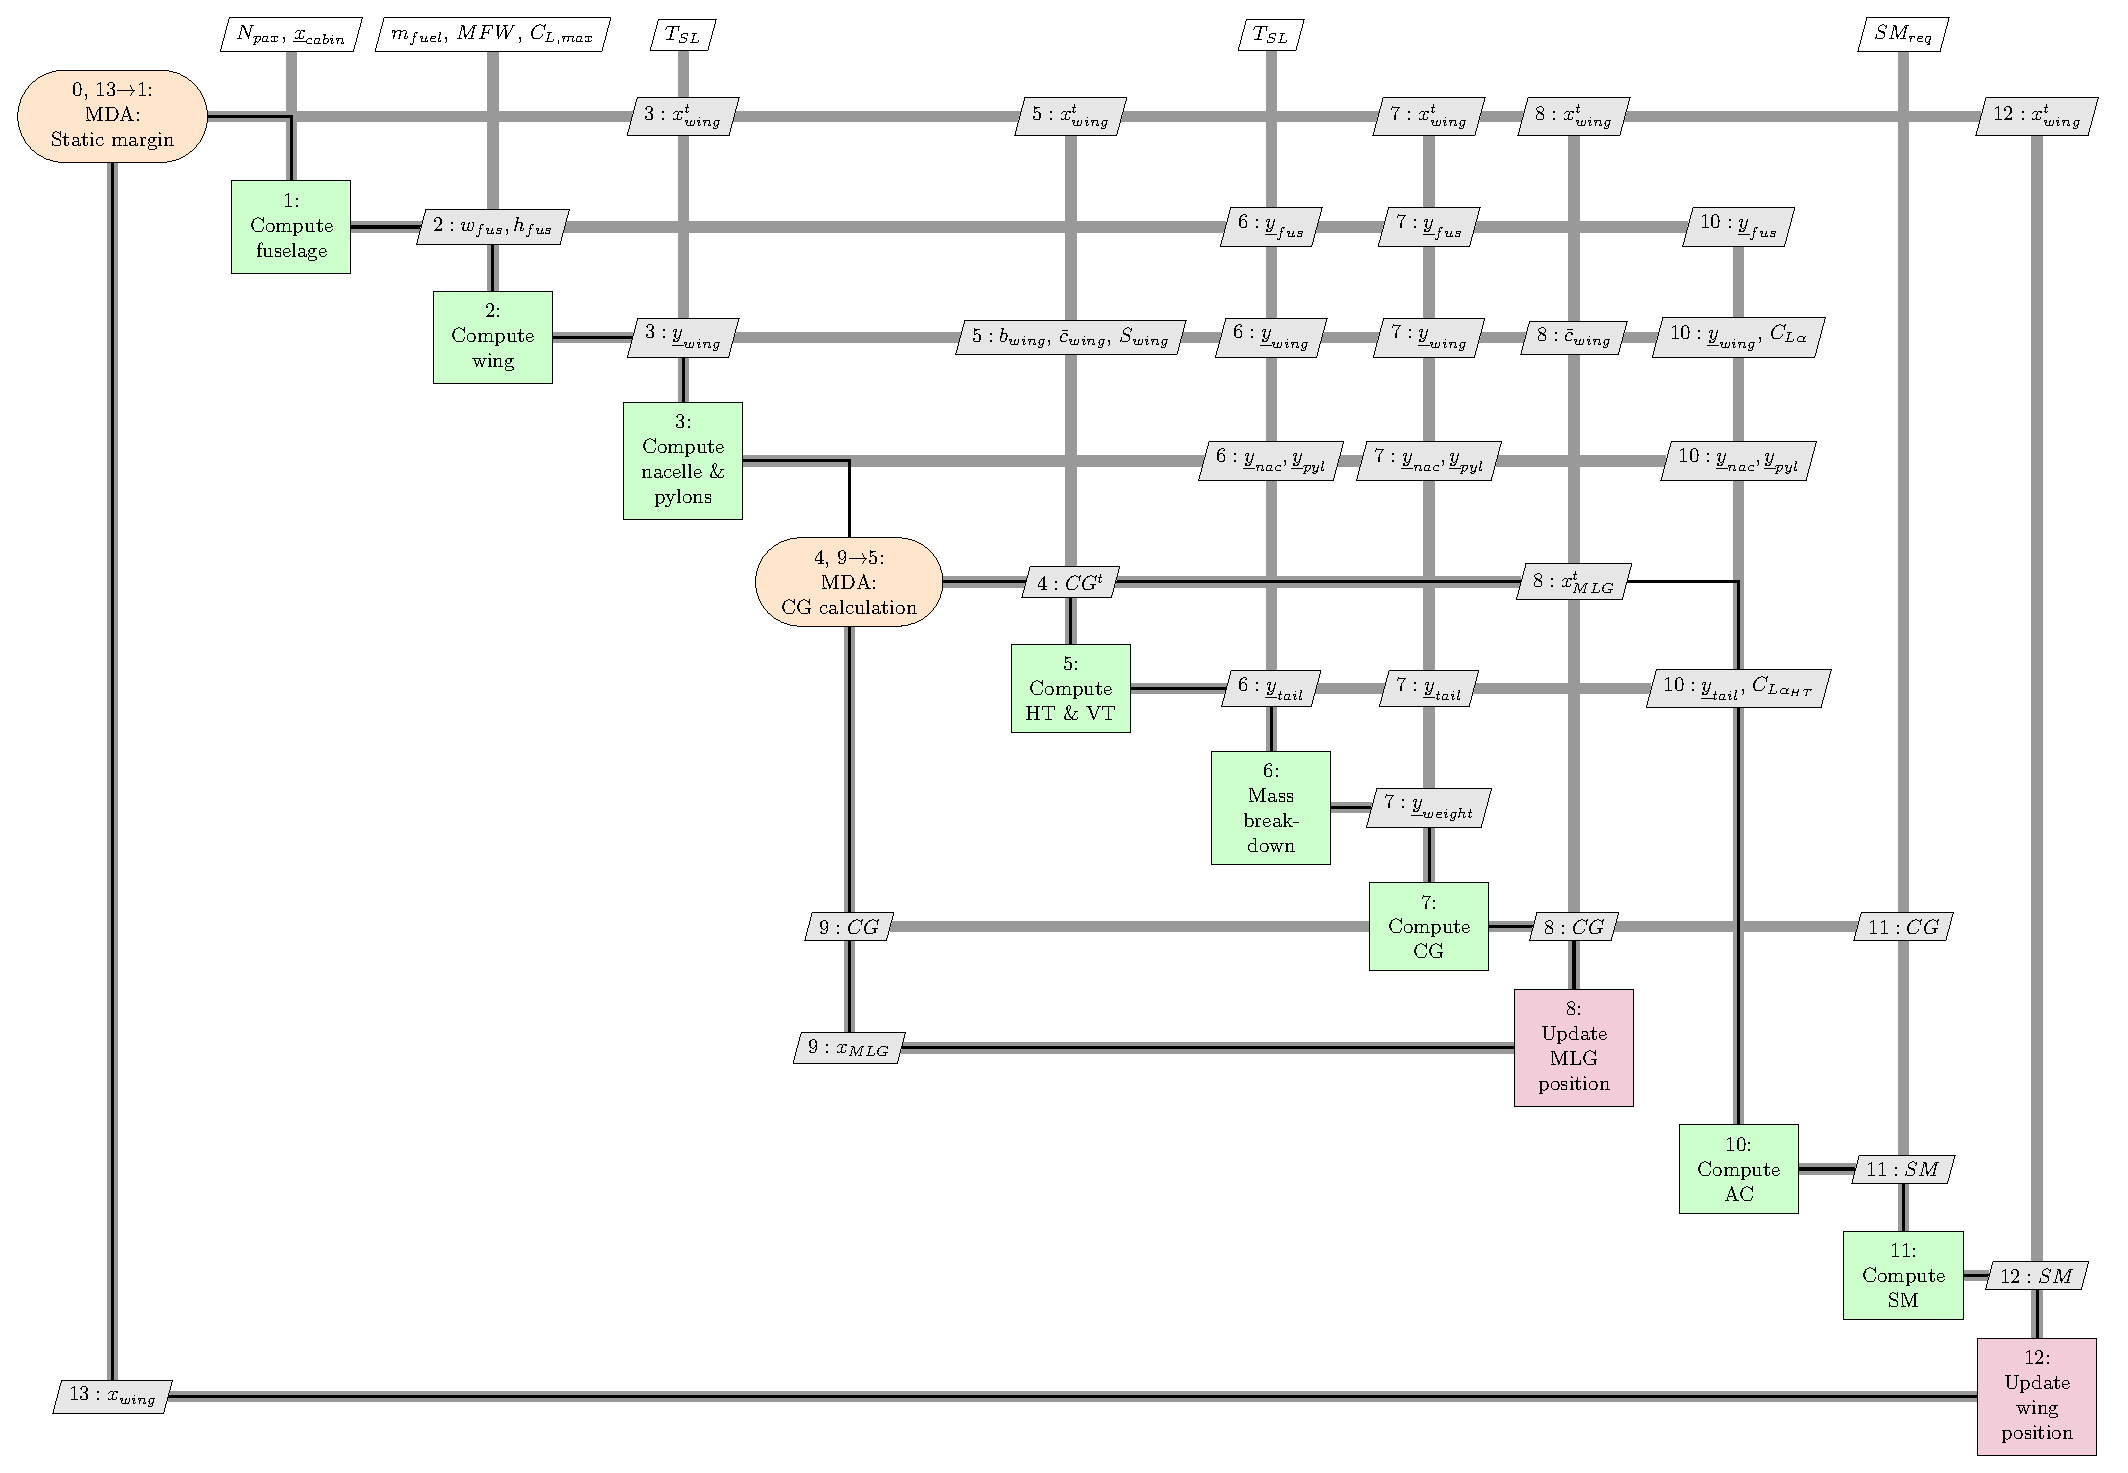
\includegraphics[keepaspectratio, width=1.2\textwidth, angle=90]{images/chap2/FAST_geometry}
	\caption{xDSM diagram of the geometry analysis coded in FAST~\cite{bib:lambe_xdsm}.}
	\label{fig:fast_geom_basic}
\end{figure}

\begin{algorithm}[!h]
	\caption{Algorithm for the geometry module of FAST, shown in Fig.~\ref{fig:fast_geom_basic}.}
	\label{alg:fast_geometry_basic}
	\begin{algorithmic}
		\REQUIRE Geometry design parameters.
		\ENSURE Aircraft geometry, that satisfied the required stability constraint.
		\STATE 0: Initialise the geometry resizing loop.
		\REPEAT
		\STATE 1: Compute the fuselage geometry, according to the required number of passengers and seat arrangement.
		\STATE 2: Compute the wing geometry, starting from the wing area information, deduced in a previous analysis.
		\STATE 3: Compute nacelles and pylons geometry.
		\STATE 4: Initialise the internal loop, to get the center of gravity.
		\REPEAT
		\STATE 5: Compute the empennages, horizontal and vertical tails, according to stability requirements.
		\STATE 6: Estimate the masses of all the components.
		\STATE 7: Estimation of the global center of gravity.
		\STATE 8: Update the main landing gear position, to get the global center of gravity.
		\UNTIL {$9 \rightarrow 5$: internal loop has converged.}
		\STATE 10: Estimate the aerodynamics center position.
		\STATE 11: Compute the static margin with Eq.~\eqref{eq:static_margin_def}.
		\STATE 12: Change the wing position, to match the static margin requirement.
		\UNTIL {$13 \rightarrow 1$ MDA has converged.} 
	\end{algorithmic}
\end{algorithm}

The diagram of Fig.~\ref{fig:fast_geom_basic} shows evidence of two iterative loops.
The outer loop is the main one, since it describes the full resizing process and it is driven by the stability requirement: the static margin SM must be included in an allowable range, given by certification. 
It is to revise that SM is defined as the distance between the center of gravity and aerodynamics center, normalized with respect to the mean aerodynamics chord: for stability it has to be negative~\cite{bib:anderson_perfo, bib:roskam_perfo}. 
However, FAST uses the opposite convention:
\begin{equation}
\label{eq:static_margin_def}
SM = \frac{x_{ac}-x_{cg}}{\bar{c}} 
\end{equation}
then for stability SM must be positive. 
Also, it can not be too high as value, otherwise the aircraft will be too stable to be easily controlled; the allowable domain, required by certification~\cite{bib:airbus_notes} is that SM is included between 5 and 10\%:
\begin{equation}
\label{eq:static_margin_limits}
0.05 \leq \textrm{SM} \leq 0.10
\end{equation}
Static margin depends mainly on the wing position: at each iteration, once that the geometry has converged, FAST controls the value of the SM and, if it exceeds the limits, it moves the wing to match the allowable range.
Then it proceeds to next iteration. 

The internal loop involves mainly the empennages and the landing gear.
At step 4 it initialises the values of horizontal and vertical tails, starting from volume coefficient estimation~\cite{bib:anderson_perfo}. 
Then it iteratively resizes the tails to ensure that the horizontal tail provides enough lift to balance the aircraft at the maximum center of gravity forward position (in the most penalizing conditions) and to respect condition given by Eq.~\eqref{eq:static_margin_limits}, and the vertical tail provides enough lateral force in cruise, to counterbalance the unstable yaw moment generated by the fuselage. 
These rules come from the work of Raymer~\cite{bib:raymer} and Kroo~\cite{bib:kroo_2001}.
At this point, the geometry module proceeds to the center of gravity estimation: in case it is out of the required range of variation, it updates the main landing gear position to fix it, to proceed at the next iteration, otherwise it proceeds with the SM estimation. 
The iterative loops give as output a viable geometry, starting from which the aerodynamics and the performances can be evaluated.

Finally, even if the wing area is computed outside this procedure, it is useful to spend some words on how it is calculated.
Its estimation is done at step 2 of Fig.~\ref{fig:fast_basic}, according to two requirements approach speed and fuel capacity. 
The first condition ensures that the wing area provides enough lift in approach, with flap and slat fully retracted, and can be represented by the lift equation as follow:
\begin{equation}
\label{eq:wing_approach_condition}
m_{L}g = \frac{1}{2}\rho V_{app}^2 S_{w_{app}} C_{L_{\max}}
\end{equation}
where $m_{L}$ is the maximum landing gear, $V_{app}$ the approach speed (23\% higher than the stall speed), $C_{L_{\max}}$ the maximum lift coefficient with flap and slat in landing configuration, and $S_{w_{app}}$ the minimum wing area needed to satisfy the equation. 

The second condition ensures that the wing is large enough to accomodate the fuel needed to complete the design mission. 
An estimation of wing capacity is provided by Raymer~\cite{bib:raymer}:
\begin{equation}
\label{eq:wing_fuel_condition}
m_{f_{\max}} = 224 S_{w_{f}}^{1.5}AR^{-0.4}\left[0.6\left(\frac{t}{c}\right)_{root}+0.4\left(\frac{t}{c}\right)_{tip}\right]+1570
\end{equation}
where $AR$ is the aspect ratio, $\frac{t}{c}$ is the thickness-to-chord ratio, evaluated at the wing root and tip, and $S_{w_{f}}$ the wing area. 
Imposing $m_{f_{\max}}=m_f$ yields to an estimation of the minimum wing area needed for the fuel storage.

The final wing area must respect both Eq.~\eqref{eq:wing_approach_condition} and Eq.~\eqref{eq:wing_fuel_condition}.
Thus the maximum value between the two estimations is chosen.
This procedure ensures a feasible value of wing area, however it is to note that it limits the exploration of the wing area to only two values, whereas the conditions described by Eq.~\eqref{eq:wing_approach_condition} and Eq.~\eqref{eq:wing_fuel_condition} may be written as inequalities, enlarging the values to explore that satisfy the conditions. 
As a conclusion, the estimated value may not be optimal, because of the limited design space, and FAST does not explore any other values but $S_{w_{app}}$ and $S_{w_{f}}$.

\subsubsection{Aerodynamics}
\label{subsubsec:chap2_fast_aero}

The aerodynamics module is devoted to the polar estimation $C_D=f\left(C_L\right)$, both for low and high speed. 
This analysis too is based on statistical and engineering equations~\cite{bib:airbus_notes}, enabling extremely fast computations
The drag coefficient is composed of three terms: friction drag $C_{D_{0}}$, induced drag $C_{D_{i}}$ and compressibility drag $C_{D_{c}}$.

Friction drag is the term due to the form, generally it does not depend by the flight condition and then is considered constant with the lift coefficient.
The formulation used in FAST depends solely on the wetted areas. 
First the friction coefficient is computed, with the Prandtl-Schlichting correlation~\cite{bib:monaghan}:
\begin{equation}
\label{eq:friction_coefficient}
c_f = \frac{0.455}{\left(1+0.126M^2\right)\left(\log_{10}Re\right)^{2.58}}
\end{equation}
where $M$ is the actual Mach number, $Re$ the Reynolds number. 
Then, the $C_{D_0}$ is computed as the sum of friction coefficients for each component:
\begin{equation}
\label{eq:cd0}
C_{D_{0}}=\sum_{i}c_{f_{i}}k_{f_{i}}\frac{S_{i_{wet}}}{S_w}
\end{equation}
where $c_{f_{i}}$ is the local friction coefficient, $S_{i_{wet}}$ the wetted surface of $i$-th component, and $k_{f_{i}}$ a corrective factor, to consider secondary aspects, such as the sweep effect. 
Note that the Reynolds number used in Eq.~\eqref{eq:friction_coefficient} is not constant, but varies for each component, since the reference length is different. 
The value of $C_{D_{0}}$ is corrected, to include a parasite drag effect, with a corrective factor depending on the total wetted area. 

The second term of the induced drag depends on the square lift coefficient, in agreement with Prandtl theory~\cite{bib:cdn_notes, bib:anderson_aero}, and it represents the greater contribution in the drag breakdown. 
It is computed as
\begin{equation}
\label{eq:cd_induced}
C_{D_{i}}= \frac{C_L^2}{\pi \left(AR\right) e}
\end{equation}
where $e$ is the Oswald factor, depending solely on the wing geometry and the Mach number, estimated using the method proposed by Ni\c{t}\u{a} and Scholz~\cite{bib:nita}. 

The induced drag is associated to the energy dissipated by the vortex at the wing trailing edge. 
These vortex generate a downwash, which must be taken into account in the drag calculation, and as well as in the needed deflection to trim the aircraft. 
This last effect generates a new source of drag, associated to trim, that is added to the induced drag and, at first istance, is computed as
\begin{equation}
\label{eq:cd_trim}
C_{D_{trim}}= 5.89\times 10^{-4} C_L
\end{equation}

Finally, the last term $C_{D_{c}}$ is associated to the presence of compressibility phenomena and shock wave on the wing. 
At low speed, it can be neglected, but in the transonic regime it is crucial to have a proper estimation of this term. 
Unfortunately, it is not an easy task to find a simple suited model, as it depends on multiple factors: Mach number, lift coefficient, wing geometry, but also flow properties. 
A good correlation is found in the Airbus notes, in which $C_{D_{c}}$ depends solely on the Mach number and $C_L$, as shown in Fig.~\ref{fig:cd_comp_example}, for a wing sweep of 28~\si{\deg} and a thickness-to-chord ratio of 12\%.
It must be noted that the tendencies vary from aircraft to aircraft; however, in the zone of interest for the flight of subsonic turbofan aircraft ($M=0.7-0.8$), the term is small and near zero, and thus the approximation works fine, despite the limitations. 
\begin{figure}[!h]
	\centering
	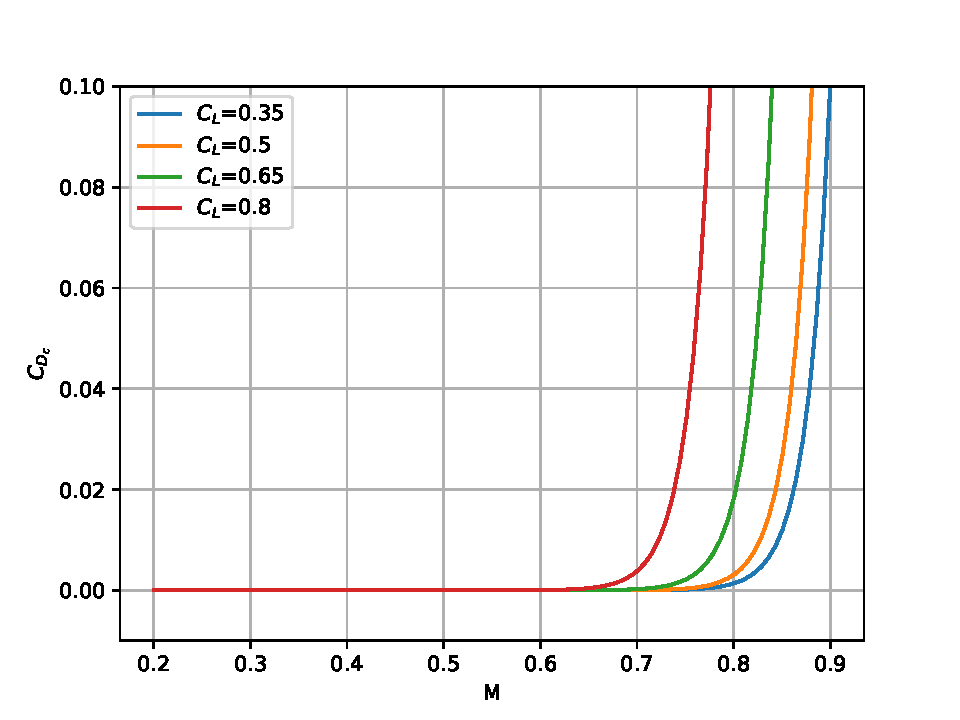
\includegraphics[keepaspectratio, width=0.7\textwidth]{images/chap2/cd_comp}
	\caption{Compressibility drag coefficient as function of Mach and lift coefficient. Curves are obtained considering $\Lambda_{25_{w}}$=28~\si{\deg} and $\left(\frac{t}{c}\right)_w$=0.12.}
	\label{fig:cd_comp_example}
\end{figure}

With all the terms are identified, the drag polar is computed as
\begin{equation}
\label{eq:cd_total}
C_D = k_{C_{D}}\left(k_{C_{D_{0}}}C_{D_{0}} + k_{C_{D_{i}}}C_{D_{i}} + k_{C_{D_{c}}} C_{D_{c}}\right)
\end{equation}
The $k$-terms are added to consider some improvements coming from the technologies, \textit{i.e.} the winglet design impact the induced drag, and this can be modeled using $k_{C_{D_{i}}}$. 

Alternatively to these equations, if desired, it is possible to use OpenVSP~\cite{bib:openvsp} for the calculations.
This code relies upon the VLM method, which is limited to incompressible flow, thus it is used only for low speed calculation, to get the slope $C_{L_{\alpha}}$ and the lift coefficient at zero angle of attack $C_{L_{0}}$. 
In real, VLM is limited to inviscid flow too, but OpenVSP offers a correction based on wetted areas.
FAST interfaces also with XFoil~\cite{bib:xfoil} for the airfoil aerodynamics, mainly used in the estimation of the maximum $C_L$ at low speed. 
To account for the three-dimensionality introduced by the sweep, the cosinus law is considered~\cite{bib:abbott, bib:cdn_notes, bib:anderson_aero}:
\begin{equation}
\label{eq:cl_max_3d}
C_{L_{\max}} = k_{w}C_{l_{\max}}\cos\Lambda_{25_{w}}
\end{equation}

\subsubsection{Mass estimation}
\label{subsubsec:chap2_fast_mass}

The mass breakdown used in FAST follows the French standard 2001/B~\cite{bib:mass_breakdown}, which is reported in Table~\ref{tab:mass_breakdown_standard} for sake of clarity. 
The OWE is divided into five parts: airframe, propulsion, systems, operational items and crew.
Adding payload and fuel, the MTOW is obtained. 
\begin{table}[!h]
	\centering
	\begin{tabular}{l l}
		\hline
		\textbf{A} & \textbf{Airframe} \\
		A1 & Wing \\
		A2 & Fuselage \\
		A3 & Horizontal and Vertical tail \\
		A4 & Flight controls \\
		A5 & Landing gear \\
		A6 & Pylons \\
		A7 & Paint \\
		\textbf{B} & \textbf{Propulsion} \\
		B1 & Engines \\
		B2 & Fuel and oil systems \\
		B3 & Unusable oil and fuel \\
		\textbf{C} & \textbf{Systems and fixed installations} \\
		C1 & Power systems (APU, electrical and hydraulical system) \\
		C2 & Life support systems (Pressurization, de-icing, seats, ...) \\
		C3 & Instrument and navigation \\
		C4 & Transmissions \\
		C5 & Fixed operational systems (radar, cargo hold mechanization) \\
		C6 & Flight kit \\
		\textbf{D} & \textbf{Operational items} \\
		D1 & Cargo equiment \\
		D2 & Passenger seats \\
		D3 & Catering equipment \\
		D4 & Passenger safety equipment \\
		D5 & Cabin toilet equipment \\
		\textbf{E} & \textbf{Crew} \\
		\textbf{F} & \textbf{Fuel} \\
		\textbf{G} & \textbf{Payload} \\		
		\hline
	\end{tabular}
	\caption{Mass breakdown standard, according to the French norm 2001/B~\cite{bib:mass_breakdown} and implemented in FAST.}
	\label{tab:mass_breakdown_standard}
\end{table} 

For parts B, C, D, and E statistical equations, reliable for standard TAW configugrations, are used.
The airframe part is the most complicated, since in general the components need to satisfy different critical conditions, according to certification. 
As example, the wing is sized to carry out the aerodynamics load, but also to limit the torsion and the bending moment and avoid aeroelasticity issues; fuselage instead needs to carry on the pressurization load, and pass the stress analyses~\cite{bib:megson}. 
Generally, for these parts, FEM or even experimental tests are used; thanks to the experience gained throughout the years, surrogate models have been developed: they are accurate as far as the configuration does not change from the TAW. 
These models, collected in the Airbus note~\cite{bib:airbus_notes}, are implemented in FAST. 

To consider the impact of different technologies, notoriously the use of new materials like composite or advanced alluminium alloy, the same technique based on the corrective factors $k$ is used: each element listed in Table~\ref{tab:mass_breakdown_standard} has its own $k$-factor, to model a reduction or increase in mass (in percentage), as proposed by Kirby~\cite{bib:kirby}.

\subsubsection{Performance}
\label{subsubsec:chap2_fast_perfo}

The performance analysis is based on the point mass approach: the aircraft is represented as a mass point, and the mission over the time is computed through a time step integration. 
For each time step, the code carries out the following analyses:
\begin{enumerate}
	\item First, the actual atmospheric data, starting from the actual altitude, are computed using the ISO standard atmosphere.
	
	\item Then, using the lift equation FAST computes the actual value of $C_L$:
	\begin{equation}
	\label{eq:lift_equation}
	C_L = \frac{mg}{\frac{1}{2}\rho V^2 S_w}.
	\end{equation}
	The drag coefficient $C_D$ is obtained interpolating the polar data with the actual value of $C_L$.
	
	\item As third step, performance analysis computes the actual propulsive data. 
	In case of balanced longitudinal flight (that is, during the cruise leg), the thrust required is already known imposing that the aircraft has no climb angle: 
	\begin{equation}
	\label{eq:balanced_flight}
	\left\{\begin{array}{l}
	L = mg \\
	D = T
	\end{array}\right.
	\end{equation} 
	In case of non balanced flight (that is, when the aircraft is climbing or descending), the thrust is obtained interpolating the engine deck on a given thrust rate, and the climb angle is computed solving the non balanced longitudinal flight equations:
	\begin{equation}	
	\label{eq:non_balanced_flight}
	\left\{\begin{array}{l}
	L\cos\gamma = mg \\
	D = T + L\sin\gamma	
	\end{array}\right.	
	\end{equation}
	In both cases, the SFC is calculated, to consider the mass variation.
	
	\item Finally, FAST updates the state vector recomputing the new value of velocity and mass
	\begin{equation}
	\label{eq:mass_perfo_update}
	m_{i+1} =  m_i - \textrm{T}(\textrm{SFC})\Delta t
	\end{equation}
	and proceeds to next iteration, using the new state vector as initial point of the following time step.
\end{enumerate}

This process can be schematised using an xDSM diagram, as shown in Fig.~\ref{fig:fast_mission_segment}.
\begin{figure}[!h]
	\centering
	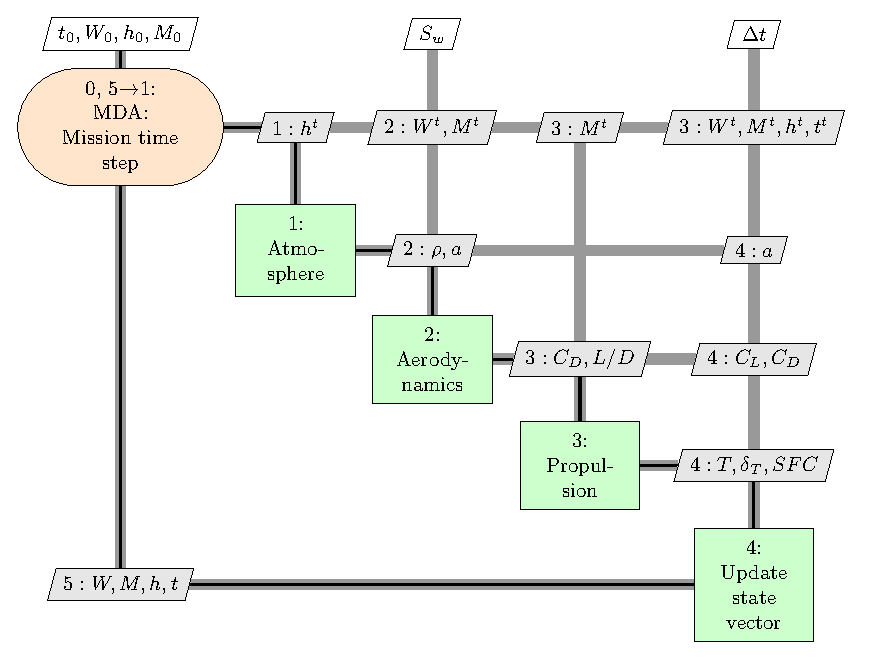
\includegraphics[keepaspectratio, width=0.6\textwidth]{images/chap2/FAST_mission_segment}
	\caption{xDSM diagram for the time step performance analysis.}
	\label{fig:fast_mission_segment}
\end{figure}

This routine allows to get a detailed trajectory. 
The mission is made up by takeoff, initial climb up to 1500~ft, climb to reach the cruise altitude, cruise, descent, an alternate flight plus holding phase to consider reserve calculation, and finally landing. The cruise altitude is found imposing that the initial point corresponds to the maximum lift-to-drag ratio; then it is possible to choose between two cruise phases: a conventional step climb and a cruise climb approach. 
They are shown in Fig.~\ref{fig:mission_profile}.
\begin{figure}[!h]
	\centering
	\begin{subfigure}{0.8\textwidth}
		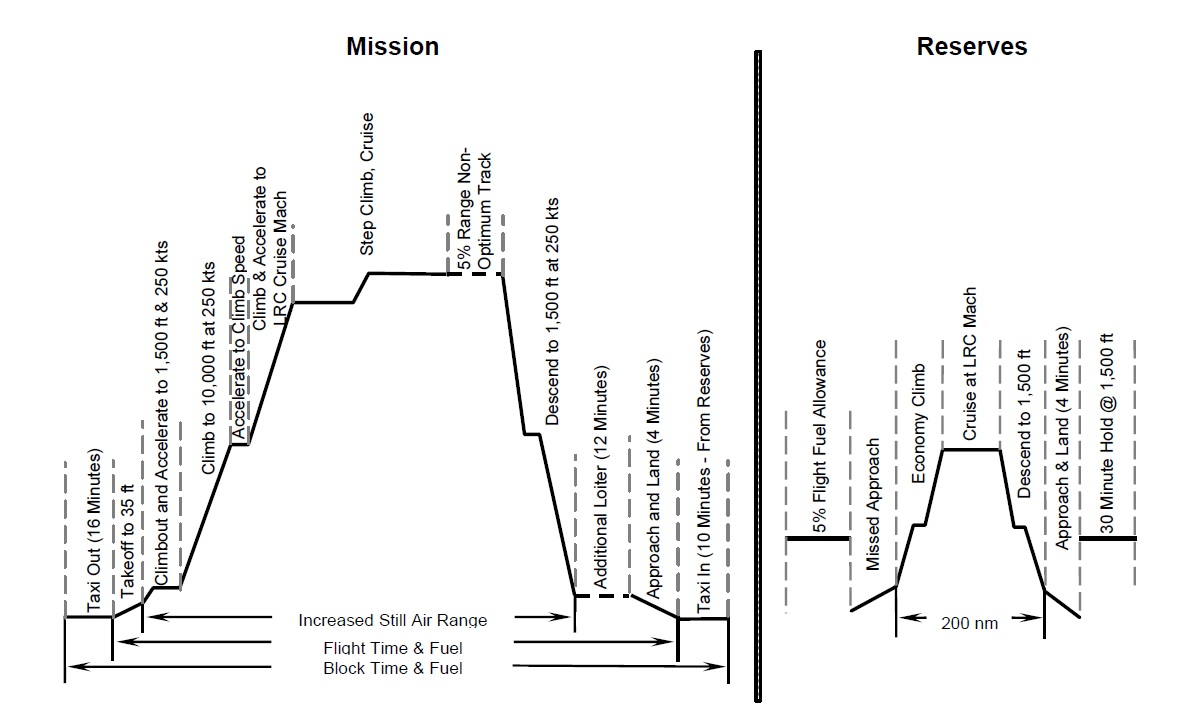
\includegraphics[keepaspectratio, width=\textwidth]{images/chap2/step_climb.jpg}
		\caption{Step climb mission.}
		\label{subfig:step_climb}
	\end{subfigure}
	\begin{subfigure}{0.8\textwidth}
		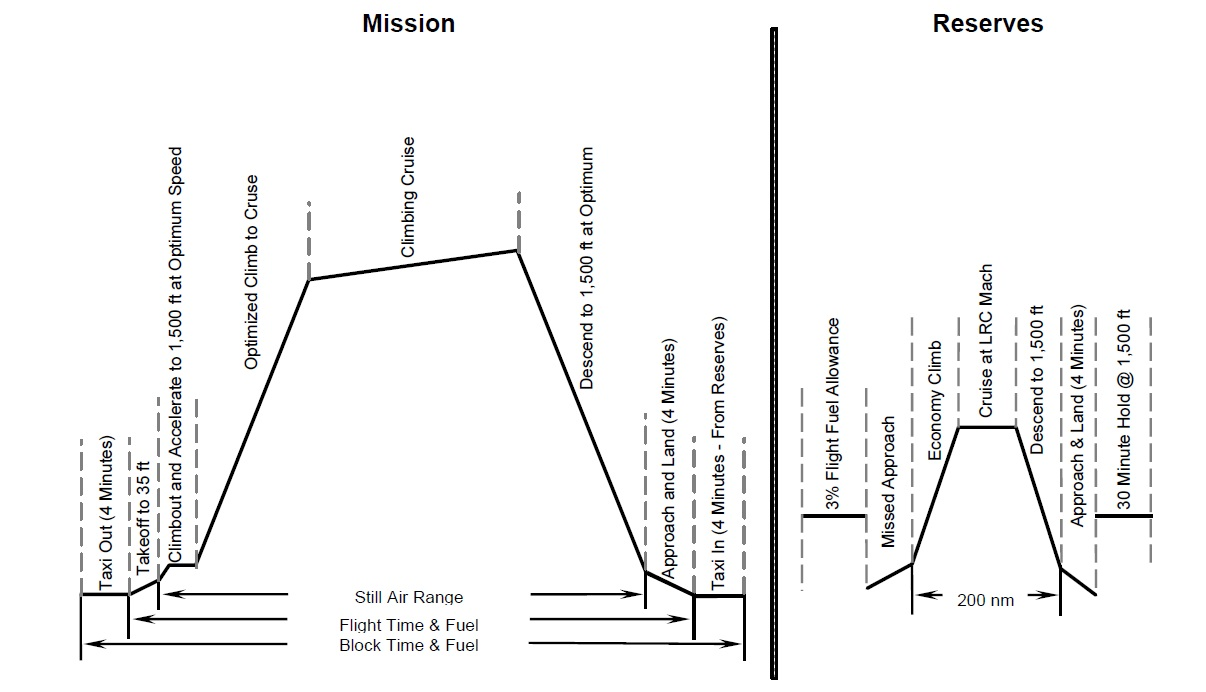
\includegraphics[keepaspectratio, width=\textwidth]{images/chap2/cruise_climb.jpg}
		\caption{Cruise climb mission.}
		\label{subfig:cruise_climb}
	\end{subfigure}
	\caption{Different mission profiles~\cite{bib:bradley_sugar_p1}.}
	\label{fig:mission_profile}
\end{figure}

The step climb approach recalls the real aircraft trajectory, for which it is mandatory to fly on predefined flight level according to the air traffic management rules~\cite{bib:mission_path_def}. 
The step climb is done only if it advantageous for fuel saving, otherwise the aircraft continues on the same level. 
However, according to NASA perspectives~\cite{bib:bradley_sugar_p1}, the cruise climb option will replace the step climb, since it requires that the aircraft always flies at its maximum lift-to-drag ratio, saving fuel. 
This new mission is also included as one of the most innovative aspects in the new air traffic management rules for a more sustainable aviation~\cite{bib:bradley_sugar_p1}.
From a coding point to view, the cruise climb approach is less time consuming than the step cruise, since at each iteration the code does not need to check if it is advantageous to perform a climb of 2000~ft.

When in the cruise leg, the descent function is called at each time step, to know the total distance travelled: in case this value is below the range, it proceeds to a new time step. 
This algorithm is not efficient, as the descent function is called many times (about 1000). 
This point is identified as an area of improvement for FAST. 
The procedure is also shown in Fig.~\ref{fig:fast_performance_basic} and described in Algorithm~\ref{alg:fast_performance_basic}, to better highlight the point. 
For clarity, only the two iterative loops, to find the cruise altitude and to cover the range, are shown; a complete diagram must include ground operation before the climb and reserve calculation after the descent. 
\begin{figure}[!h]
	\centering
	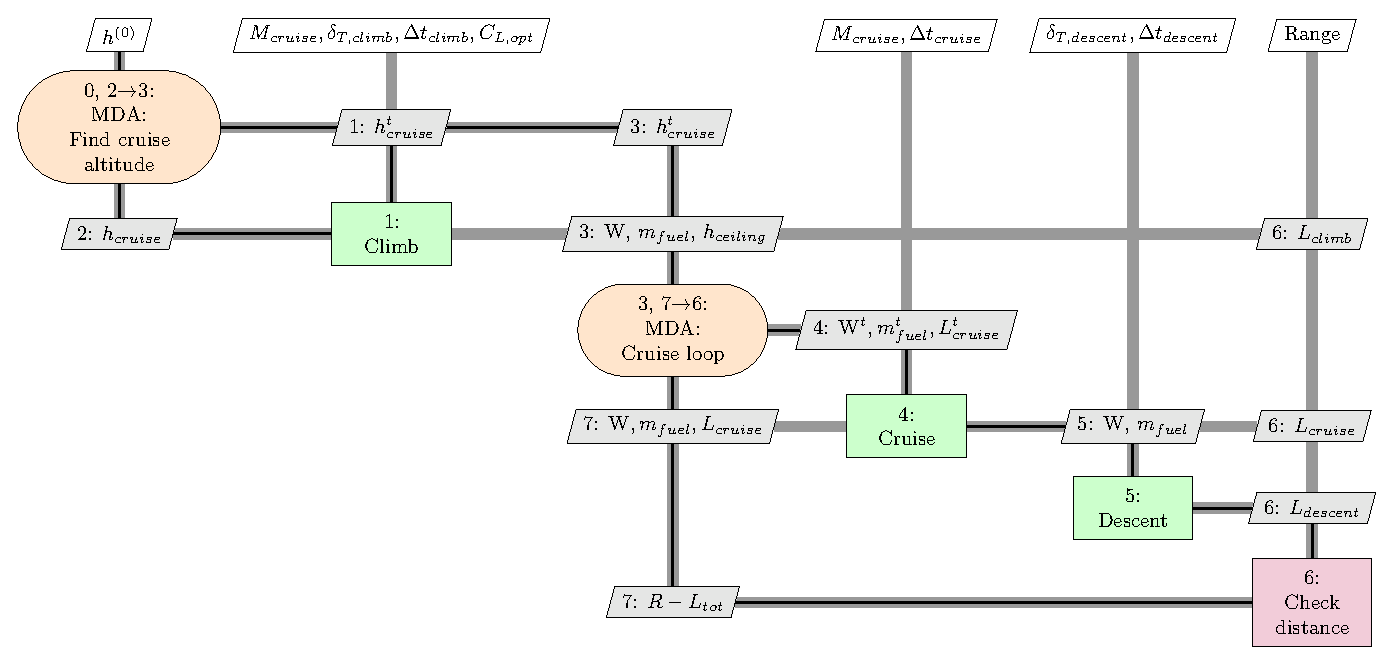
\includegraphics[keepaspectratio, width=\textwidth]{images/chap2/FAST_performance}
	\caption{xDSM diagram climb and cruise phase performance, to highlight the iterative procedure used in FAST.}
	\label{fig:fast_performance_basic}
\end{figure}

\begin{algorithm}[!h]
	\caption{Algorithm for climb and cruise phase performance, with reference to xDSM diagram shown in Fig.~\ref{fig:fast_performance_basic}.}
	\label{alg:fast_performance_basic}
	\begin{algorithmic}
		\REQUIRE MTOW and polar.
		\ENSURE Detailed trajectory calculation.
		\STATE 0: Initialise the climb loop.
		\REPEAT
		\STATE 1: Compute the climb and check if the final altitude corresponds to the maximum lift-to-drag ratio.
		\STATE 2: If the final climb altitude does not correspond to that of maximum lift-to-drag ratio, compute a new value, otherwise proceed to next iteration.
		\UNTIL {$2 \rightarrow 1$: initial cruise altitude is found.}
		\REPEAT
		\STATE 3: Initialise the state vector for the cruise phase.
		\STATE 4: Perform a time step of cruise leg.
		\STATE 5: Compute the descent leg.
		\STATE 6: Compute the difference between the required range and the total distance travelled.
		\STATE 7: Check if the difference of step 6 is equal to zero: if not, proceed to a new time step.
		\UNTIL {$7 \rightarrow 1$ total required range is covered.} 
	\end{algorithmic}
\end{algorithm}

\subsubsection{CCM -- Certification Constraint Module}
\label{subsubsec:chap2_ccm}

The Certification Constraints Module, abbreviated as CCM by now, is the module developed by Schmollgruber during his Ph.D.~\cite{bib:schmollgruber, bib:schmollgruber_phd}. 
The scope of the CCM is to check if certification specifications are respected: indeed, it is not sufficient that the aircraft is viable, but it must comply with the EASA/FAA rules.

The module works outside the sizing loop: it limits to control if the aircraft complies with certifications, but in case one of the rules is not satisfied, it does not proceed by itself to any correction. 
It is up to the user to go back manually and change the design parameter to get the certifications satisfied.
However, it may be integrated within an optimisation loop, where the conditions are design constraints, and the algorithm may find the optimum design that satisfies all the rules above. 
This procedure has been set by Schmollgruber, who used \texttt{Scipy} libraries to carry out an optimisation based on certifications~\cite{bib:schmollgruber_phd}.

The CCM module relies upon a \texttt{xml} file, which contains the prescribed conditions to check, using the meta-model GAMME as for the I/O file~\cite{bib:bedouet}.
The documents considered are the CATPOL~\cite{bib:catpol} and CS-25~\cite{bib:cs25}, that are related to large passenger aircraft and prescribe the conditions to be respected en-route and during takeoff and landing (the most stringent segments), with all engines operative and in case of failure. 
For each case, the CCM solves the flight equations using the Python function \texttt{fsolve}.
The details of rules are listed below; for shortness the acronym AEO is used to indicate the condition of all engine operative, and OEI to indicate the one engine inoperative condition. 
\begin{itemize}
	\item \textbf{CAT.POL.A.410(a)}. This paragraph of the CATPOL document~\cite{bib:catpol} prescribes that, in en-route condition with all the engines operative, at the top of climb (1) and top of descent (2) the aircraft must preserve a reserve of vertical speed not below than 300~ft/min.
	
	\item \textbf{CS-25.119(a)}. This rule, from CS-25 specifications for large passenger aircraft~\cite{bib:cs25}, requires that in landing condition with AEO, the steady gradient flight must not be less than 3.2\%.
	
	\item \textbf{CS-25.121(a)}. This rule requires that, during takeoff with landing gear extracted and OEI condition, the steady gradient flight must be positive. 
	
	\item \textbf{CS-25.121(b)}. This rule requires that, during takeoff and OEI condition, at the point of flight path when the landing gears are fully retracted (400~ft), the steady gradient flight must not be less than 2.4\%.
	
	\item \textbf{CS-25.121(c)}. This rule requires that, in en-route configuration at the end of takeoff and in OEI condition, the steady gradient flight must not be less than 1.2\%.
	
	\item \textbf{CS-25.121(d)}. This rule requires that, in approach configuration with AEO condition, the steady gradient flight must not be less than 2.1\%.
\end{itemize} 

Table~\ref{tab:ccm_rules} sums up the rules, together with the flight path specified and the minimum value of parameters required. The notation $V_{z}$ indicates the vertical speed, meanwhile $\gamma_{\%}$ the steady gradient flight in percentace.
\begin{table}[!h]
	\centering
	\begin{tabular}{l c c c c}
		\hline
		\textbf{Certification} & \textbf{Phase} & \textbf{Condition} & \textbf{Parameter} & \textbf{Min. value} \\
		\hline
		CAT.POL.A.410(a)-1 & Top of climb & AEO & $V_{z}$ & 300~ft/min \\
		CAT.POL.A.410(a)-2 & Top of descent & AEO & $V_{z}$ & 300~ft/min \\
		CS-25.119(a) & Landing & AEO & $\gamma_{\%}$ & 3.2~\% \\
		CS-25.121(a) & Takeoff & OEI & $\gamma_{\%}$ & 0~\% \\
		CS-25.121(b) & 400~ft & OEI & $\gamma_{\%}$ & 2.4~\% \\
		CS-25.121(c) & End of takeoff & OEI & $\gamma_{\%}$ & 1.2~\% \\
		CS-25.121(d) & Approach & AEO & $\gamma_{\%}$ & 2.1~\% \\
		\hline
	\end{tabular}
	\caption{CATPOL~\cite{bib:catpol} and CS-25~\cite{bib:cs25} rules explanation, considered in the CCM module of FAST. $V_{z}$ represents vertical speed, meanwhile $\gamma_{\%}$ the gradient flight.}
	\label{tab:ccm_rules}
\end{table}

\subsection{Test case: Airbus A320}
\label{subsec:chap2_fast_test_case}

FAST has been developed for designing large passenger aircraft, using turbofan as engine. 
The validation case, presented by Schmollgruber et al.~\cite{bib:fast_main}, is the Airbus A320~\cite{bib:a320_specifications}, with the top level requirements reported in Table~\ref{tab:fast_base_tlar}.
The geometrical inputs required are instead reported in Table~\ref{tab:fast_base_geom_inp}, following the list presented in Table~\ref{tab:fast_geom_entry_parameter}.
Finally, Table~\ref{tab:fast_base_thrust_rate_entry} reports the thrust rate for each mission segment. 
\begin{table}[!h]
	\centering
	\begin{tabular}{l r r}
		\hline
		Range & 2750 & nmi \\
		Number of passengers & 150 & \\
		Approach speed & 132 & \si{\knot} \\
		Design payload & 13608 & \si{\kilogram} \\
		\hline		
	\end{tabular}
	\caption{Top level requirements for the A320 CERAS validation case used in FAST.}
	\label{tab:fast_base_tlar}
\end{table}
\begin{table}[!h]
	\centering
	\begin{tabular}{l r l}
		\hline
		$AR_w$ & 9.5 & \\
		$\Lambda_{25_{w}}$ & 25 & \si{\deg} \\
		$\lambda_w$ & 0.38 & \\
		$\lambda_{HT}$ & 0.4 & \\
		$\left(\frac{t}{c}\right)$ & 0.1 & \\
		$\lambda_{VT}$ & 0.3 & \\
		$\left(\frac{t}{c}\right)$ & 0.13 & \\
		\hline
	\end{tabular}
	\caption{Geometrical inputs for the A320 CERAS validation case.}
	\label{tab:fast_base_geom_inp}
\end{table}
\begin{table}[!h]
	\centering
	\begin{tabular}{l c}
		\hline
		Segment & $\delta_T$ \\
		\hline
		Taxi & 0.3 \\
		Takeoff & 1.0 \\
		Climb & 0.93 \\
		Cruise & Computed \\
		Descent & 0.55 \\
		Alternate climb & 0.93 \\
		Alternate cruise & Computed \\
		Alternate descent & 0.55 \\
		Hold & Computed \\
		Landing & 0.03 \\
		\hline
	\end{tabular}
	\caption{Thrust rate definition for each mission segment for the A320 CERAS validation case.}
	\label{tab:fast_base_thrust_rate_entry}
\end{table}
Actually, even if the Airbus A320 specification manual contains many geometrical information, as well as cargo disposition, it does not have any information regarding the mass breakdown, performance and the engine map. 
Thus, in FAST, the CERAS data are considered for comparison~\cite{bib:ceras}, since it emulates the Airbus A320 aircraft; engine model is direcly taken from the website. 
All the performances of this reference aircraft are available, and thus are used for the comparison. 

The results of FAST, for the A320, are shown in Fig.~\ref{fig:fast_base_results}: the climb and descent profile are depicted in Fig.~\ref{fig:fast_base_climb} and Fig.~\ref{fig:fast_base_descent}, meanwhile the global profile, using both the step cruise and the cruise climb, are shown in Fig.~\ref{fig:fast_base_cruise_step} and Fig.~\ref{fig:fast_base_cruise_climb}. 
The drag polar is reported in Fig.~\ref{fig:fast_base_polar}, while the payload range diagram of Fig.~\ref{fig:fast_base_pl_range} ends the set of output available. 
Note that the mission profile is very detailed and mimics a real aircraft trajectory, according to the air traffic rules~\cite{bib:mission_path_def}.
\begin{figure}[!h]
	\centering
	\begin{subfigure}{0.45\textwidth}
		\centering
		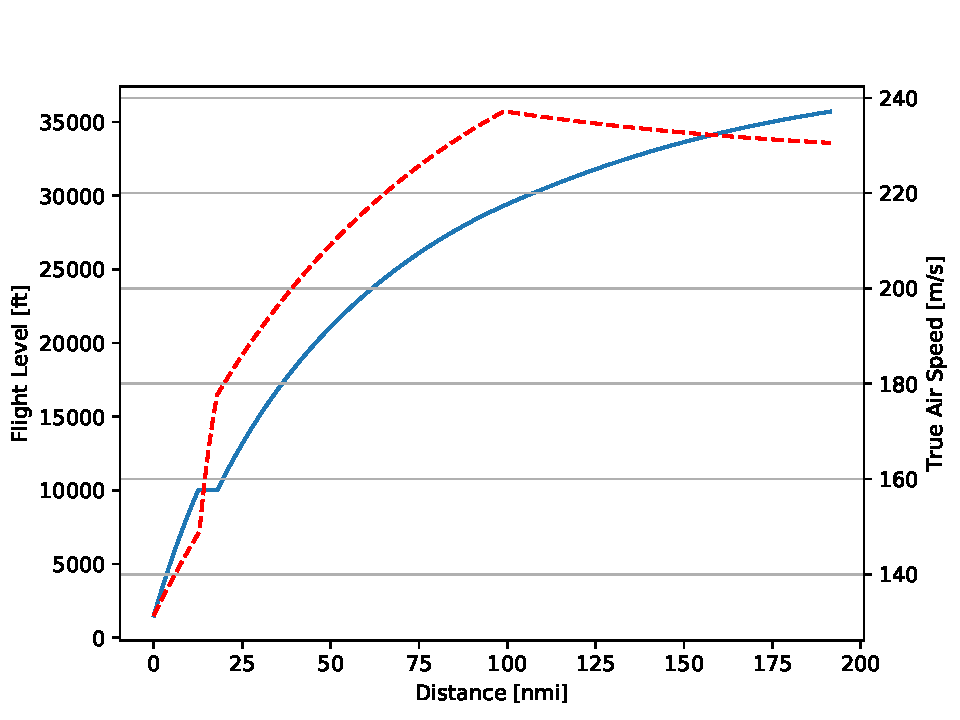
\includegraphics[keepaspectratio, width=\linewidth]{images/chap2/FAST_base_climb_profile}
		\caption{Climb profile.}
		\label{fig:fast_base_climb}
	\end{subfigure}
	\hspace{10mm}
	\begin{subfigure}{0.45\textwidth}
		\centering
		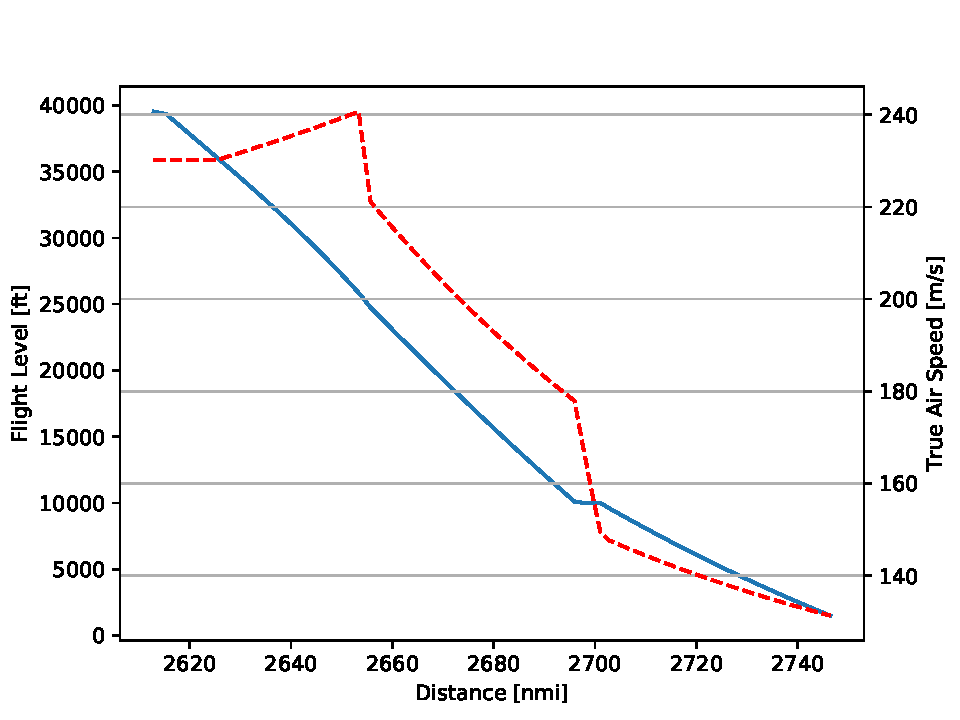
\includegraphics[keepaspectratio, width=\linewidth]{images/chap2/FAST_base_descent_profile}
		\caption{Descent profile.}
		\label{fig:fast_base_descent}
	\end{subfigure}
	
	\begin{subfigure}{0.45\textwidth}
		\centering
		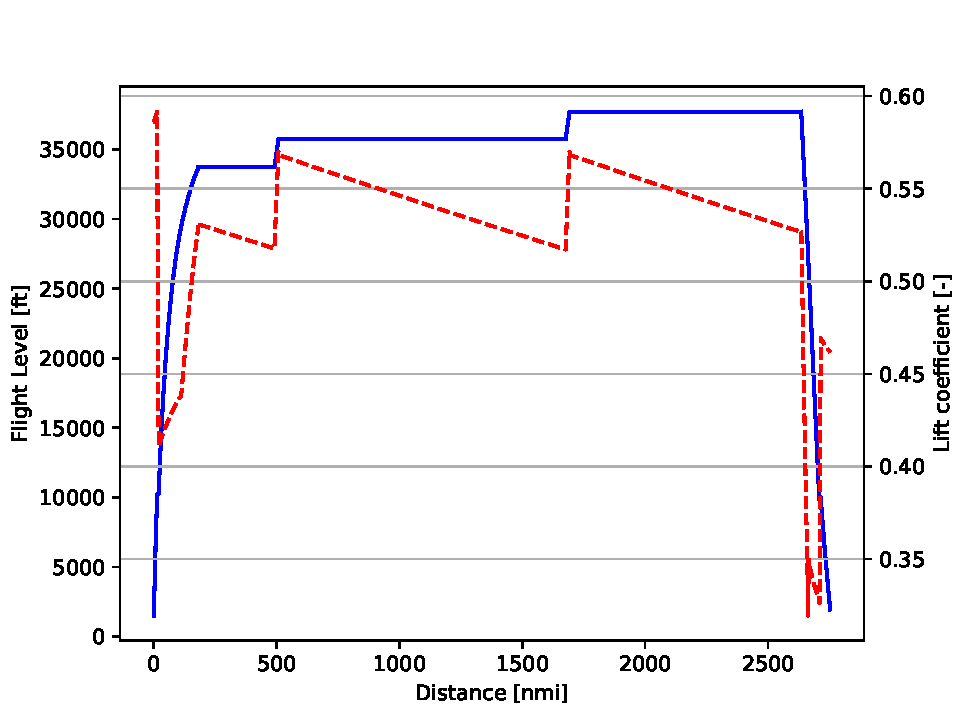
\includegraphics[keepaspectratio, width=\linewidth]{images/chap2/FAST_base_cruise_step_profile}
		\caption{Step cruise profile.}
		\label{fig:fast_base_cruise_step}
	\end{subfigure}	
	\hspace{10mm}
	\begin{subfigure}{0.45\textwidth}
		\centering
		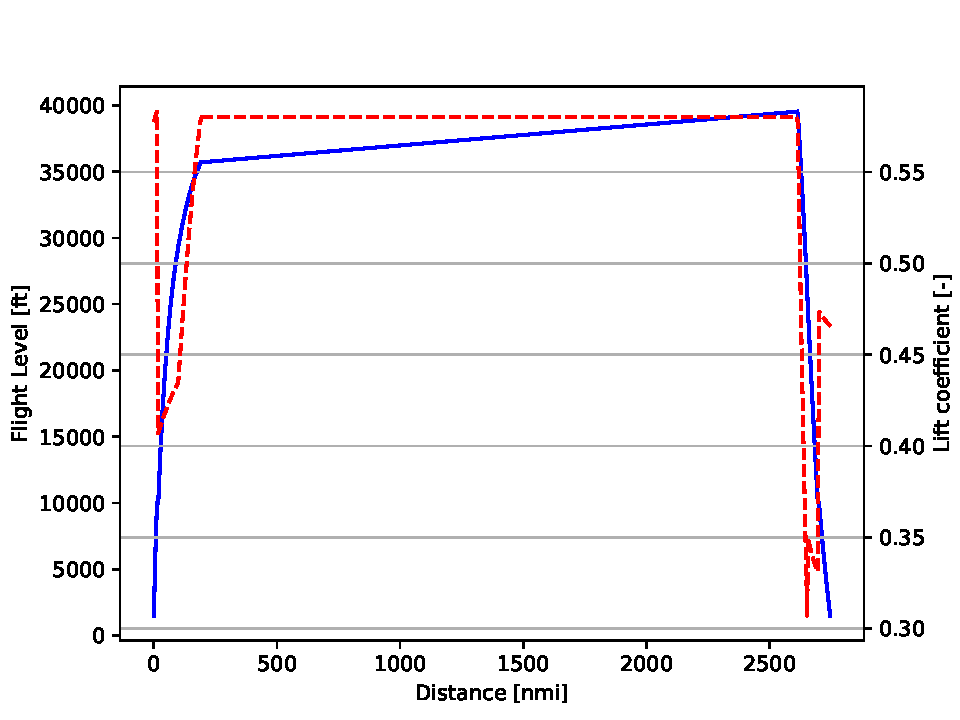
\includegraphics[keepaspectratio, width=\linewidth]{images/chap2/FAST_base_cruise_climb_profile}
		\caption{Cruise climb profile.}
		\label{fig:fast_base_cruise_climb}
	\end{subfigure}
	
	\begin{subfigure}{0.45\textwidth}
		\centering
		\includegraphics[keepaspectratio, width=\linewidth]{images/chap2/FAST_base_polar}
		\caption{Drag polar.}
		\label{fig:fast_base_polar}
	\end{subfigure}
	\hspace{10mm}
	\begin{subfigure}{0.45\textwidth}
		\centering
		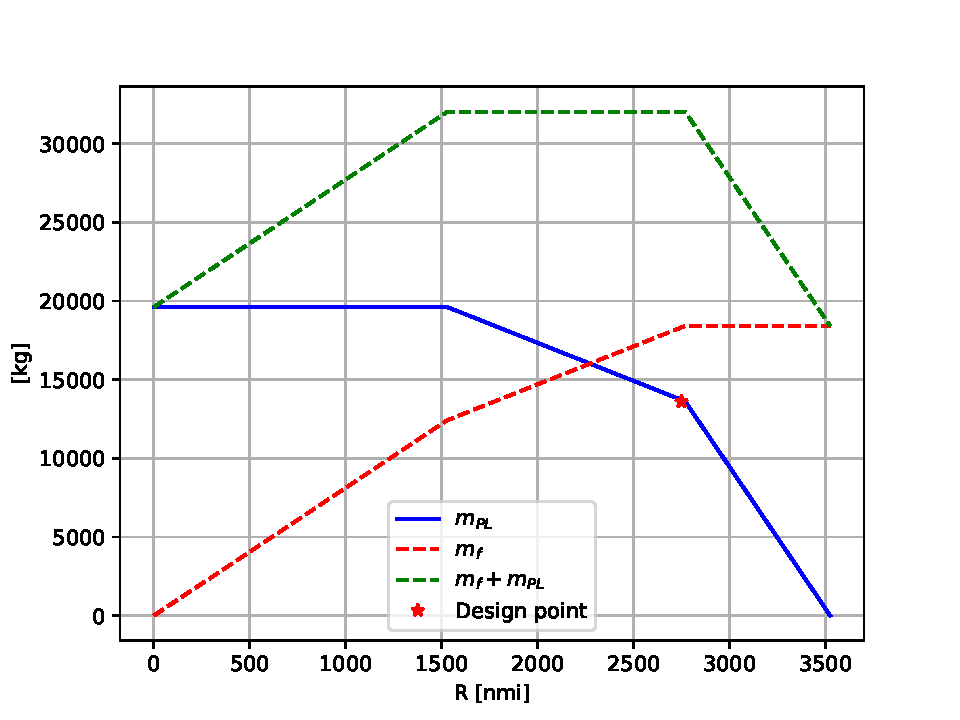
\includegraphics[keepaspectratio, width=\linewidth]{images/chap2/FAST_base_pl_range}
		\caption{Payload-Range diagram.}
		\label{fig:fast_base_pl_range}
	\end{subfigure}
	\caption{Some of the outputs of FAST, related to the A320 validation test case, with the TLAR reported in Table.~\ref{tab:fast_base_tlar}.
	Continuous line represents the trajectory, meanwhile dashed line is the true air speed or the lift coefficient, according to the flight phase.}
	\label{fig:fast_base_results}
\end{figure}

Table~\ref{tab:fast_base_comparison} reports the comparison between FAST, using both the step climb and the cruise climb approach, and the reference aircraft: it can be seen that the results are consistent, since the maximum difference is always less than 1\%. 
It must be highlighted that the step cruise and the cruise climb results are similar, but the computational cost of the second approach is reduced, because it does not need to check if it is convenient or not to perform a step of 2000~ft. 
For this reason, only this approach will be used for the future simulations. 
\begin{table}[!h]
	\centering
	\begin{tabular}{l l c c c}
		\hline
		& & \textbf{Step climb} & \textbf{Cruise climb} & \textbf{A320 CERAS} \\
		\hline
		MTOW & [\si{\kilogram}] & 74168.96 & 74562.82 & 74102.34 \\
		OWE & [\si{\kilogram}] & 42200.58 & 42190.71 & 42120.22 \\
		Wing area & [\si{\square\meter}] & 122.74 & 122.68 & 122.41 \\
		Mission fuel & [\si{\kilogram}] & 18799.11 & 18798.85 & 18678.12 \\
		\hline
	\end{tabular}
	\caption{Comparison between the results obtained in FAST and the A320 CERAS data~\cite{bib:fast_main}.}
	\label{tab:fast_base_comparison}
\end{table}

The CCM results are instead presented in Table~\ref{tab:fast_base_ccm}: the aircraft is compliant with both CATPOL and CS-25 specifications, with a safe margin for all the parameters.
The margin is taken to consider the case of hot day, with airport at high altitude (for the Airbus A320, La Paz airport is considered, which is 2000~\si{\meter} above the sea level).
\begin{table}[!h]
	\centering
	\begin{tabular}{l r l}
		\hline
		\textbf{CAT.POL.A.410(a)-1} & 964.69 & ft/min \\
		\textbf{CAT.POL.A.410(a)-2} & 1031.82 & ft/min \\
		\textbf{CS-25.119(a)} & 19.46 & \% \\
		\textbf{CS-25.121(a)} & 1.61 & \% \\
		\textbf{CS-25.121(b)} & 3.43 & \% \\
		\textbf{CS-25.121(c)} & 5.56 & \% \\
		\textbf{CS-25.121(d)} & 7.19 & \% \\
		\hline
	\end{tabular}
	\caption{CCM results for the A320 CERAS validation case.}
	\label{tab:fast_base_ccm}
\end{table}

Finally, some remarks on the computational time: the idea at the basis of FAST is to have a reliable code capable to deal with multidisciplinarity of aircraft design process and to have a result in a short time. 
The complete sizing process is done in 15-30 minutes, with the variation being associated with various TLAR and CPU performance level.
For the specific case of the reference Airbus A320 aircraft, the code runs for 25 minutes using the step climb approach and 20 minutes using the cruise climb approach. 
Preliminary tests indicated that the recoding of the cruise segment, as stated in Sec.~\ref{subsubsec:chap2_fast_perfo}, could lead to a reduction of CPU time of 5 to 10 minutes.

\section{OpenMDAO -- a multidisciplinary optimisation platform}
\label{sec:chap2_openmdao_overview}

OpenMDAO has ben created because of the need of NASA to have its own MDAO framework, in 2012, when v1.0 was released~\cite{bib:gray_omdao_2012, bib:gray_omdao_2014}. 
The code has been continuously developed throughout the years; this research considers the version 2.4, released in August 2018.~\cite{bib:openmdao_website}. 
OpenMDAO has been coded in Python, to facilitate the scripting, but also because the \texttt{Scipyoptimisation} python library already includes several optimisation algorithm, both gradient-free and gradient-based~\cite{bib:scipy_2007, bib:scipy_2011}, that can be inheritated as class by OpenMDAO. 
It also provides a class to use the \texttt{pyOptSparse} library~\cite{bib:pyopt}, which extends the gradient-based algorithms choice. 

The first feature of OpenMDAO is that it uses distributed memory and high performance computing to speed up the serial computation, as well as it enables efficient parallel execution~\cite{bib:balabanov, bib:hwang_2015}. 
Although OpenMDAO can use also algorithms not based on derivatives, the major feature of this framework is the possibility to compute total derivatives very efficiently: OpenMDAO, indeed, relies upon the unified theory MAUD developed by Hwang and Martins for the gradient calculation~\cite{bib:hwang_unif, bib:hwang_2018}. 
Users can choose among finite differences method, complex step or analytic derivatives, making the code very flexible. 
In the first two cases the code automatically computes derivatives, meanwhile in the last one the user needs to define analytic expressions within the process. 
At first a large effort in the set-up is required, but analytic derivatives speed up the process significantly. 
Several authors benchmark algorithms that use derivatives against gradient-free algorithms, and all of them show the number of iterations is reduced by several order of magnitude when considering derivatives~\cite{bib:martins_mdo, bib:yu_2018, bib:tedford}. 
Also, as general rule, the required number of iterations for gradient-free methods grow quadratically with the number of design variables, whereas the trend is linear for gradient-based methods, as also remarked in Fig.~\ref{fig:gradbas_vs_gradfree}, which represents the required number of iterations as function of design variables number for different methods.  
\begin{figure}[!h]
	\centering
	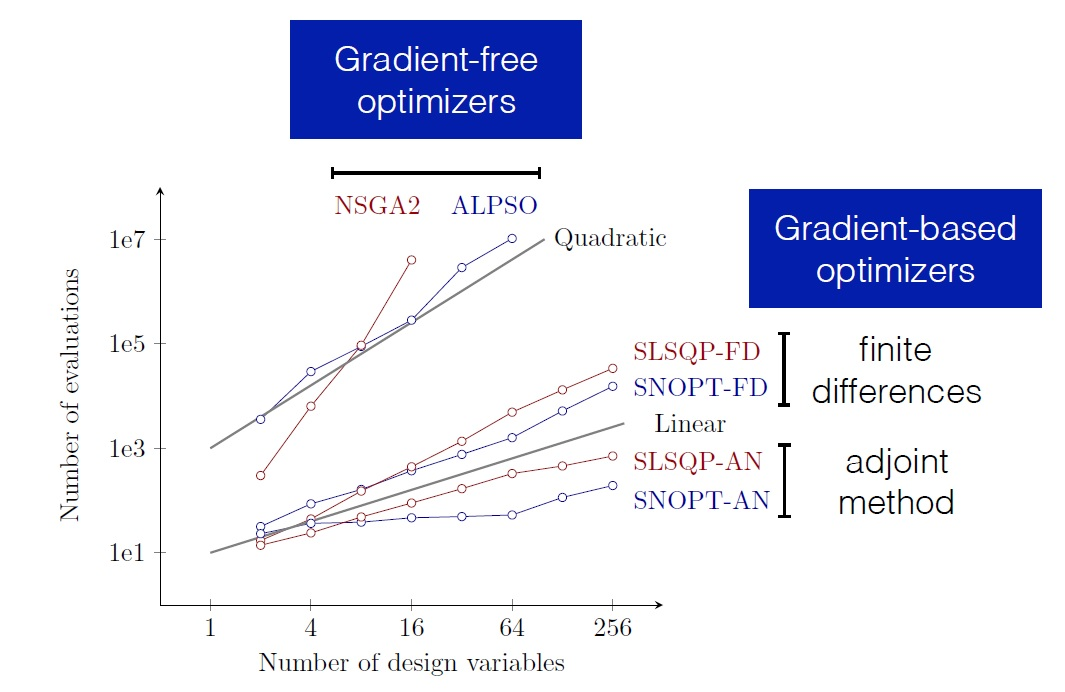
\includegraphics[keepaspectratio, width=0.8\textwidth]{images/chap2/gradbas_vs_gradfree.jpg}
	\caption{Comparison between gradient-free and gradient-based methods on the required number of iterations~\cite{bib:martins_2014}.}
	\label{fig:gradbas_vs_gradfree}
\end{figure}

The total derivatives compose a non linear system of equations which can be solved by an adjoint or a direct method. 
The solution of this system gives the path towards the function minimum. 
The usage of unified theory makes OpenMDAO perfect for large-scale problems, since it conjugates computational efficiency and multidisciplinary design~\cite{bib:hwang_omdao}. 
Also, as a consequence, the computational cost is kept low even increasing the number of disciplines in coupled high-fidelity problems~\cite{bib:martins_2005}. 
This is a key in the design of new technologies, such as BLI, since it enables to establish tradeoff in acceptable time. 

Starting from v2.4 the usage of sparse matrix has been implemented, reducing the computational cost to solve the non linear system of derivatives. 
Sparse matrices also allow to use a direct method, instead of a numerical one, in order to find the solution of the non linear system, making the code stable and easy to use by a user who does not have enough background on numerical methods, which is a non-trivial aspect.

The success of OpenMDAO as a reliable and efficient multidisciplinary optimisation platform is demonstrated by its large users community.
Problems concerning the aero-structural optimisation~\cite{bib:jasa_openaerostruct}, topology optimisation~\cite{bib:jasa_topology}, on-demand mobility~\cite{bib:hwang_x57}, small satellite design~\cite{bib:hwang_satellite}, trajectory optimisation with cost analysis~\cite{bib:hwang_mission_opt}, wind turbine blade shape optimisation~\cite{bib:barlas} and boundary layer ingestion optimisation using high fidelity~\cite{bib:gray} are succesfully solved with this framework.

In the following paragraphs, a brief description on how to use OpenMDAO is provided. 
In this manner, the integration of FAST can be better illustrated: more details about its structure, as well as the theory behind the solvers used and their implementation in the framework are given. 
OpenMDAO uses the object-oriented programming paradigm, which is facilitated by Python scripting, and an object composition design pattern. 
Just four classes are defined in OpenMDAO: \texttt{Component, Group, Driver}, and \texttt{Problem}.
They are detailed below. 

\begin{itemize}
	\item \texttt{Component} class. Components in OpenMDAO replace the classical definition of ``discipline'' in a MDO process. 
	They can represent a whole discipline, or a sub-set of it.
	Components share a common interface that allows them to be integrated to form larger problems: thus, they are the fundamental bricks in OpenMDAO to build the process.
	There are no specification about the component's instance: it simply maps a set of inputs to give a desired set of outputs, no matter if the outputs are provided with equations or a call to an external software, potentially written in a different language. 
	The \texttt{Component} class can be further divided into \texttt{ExplicitComponent} and \texttt{ImplicitComponent}: as the name suggests, the first uses explicit formulation in which the outputs are direct function of inputs; on the contrary in the second instance outputs are implicit function of inputs, and they are found through an iterative procedure that drives the function's residuals (defined by the user) to zero. 
	
	\item \texttt{Group} class. The \texttt{Group} instance contains the components, other groups, or a mix of both. 
	The relationship between groups and components forms a hierarchy tree, where a top-level group contains other groups. 
	In turn, these groups contain other groups and so on; the bottom-level contains only components. 
	There are no limit on the hierarchy level that can be defined. \texttt{Group} instances are used mainly to package sets of components together, to create better organised namespaces (since all the components are named based on their ancestors on the tree) and to facilitate the use of hierarchical nonlinear and linear solvers. 
	The ensemble of all the groups basically forms the model. 
	
	\item \texttt{Driver} class. The \texttt{Driver} instance defines a set of algorithms which iteratively call the model. 
	The algorithms are not only limited to optimisation, but can be also defined to execute other functionalities, \textit{i.e.} a sensitivity analysis or design of experiments.
	As said previously, \texttt{Driver} class already instances the \texttt{Scipyoptimisation} and the \texttt{pyOptSparse} classes, but a user can code its own class, which can be later instanciated in OpenMDAO. 
	In case of optimisation, design variables are a subset of models' inputs, objective function and eventually constraints are a subset of models' outputs. 
	
	\item  \texttt{Problem} class. This class has the function of top-level container, which includes all the objects defined. A \texttt{Problem} instance contains all the hierarchical structure, defined by groups and components, and a single driver instance. Aside of serving as a container, \texttt{Problem} class provides also the user interface for setup and execution.   
\end{itemize} 

The relationship between the four OpenMDAO classes is illustrated in Fig.~\ref{fig:omdao_class_relation}. Following the same definition given by Gray et al.~\cite{bib:gray_omdao}, ``partial derivative'' refers to the derivatives of component outputs with respect to inputs, meanwhile ``total derivative'' refers to derivatives of model outputs with respect to model inputs. 
\begin{figure}[!h]
	\centering
	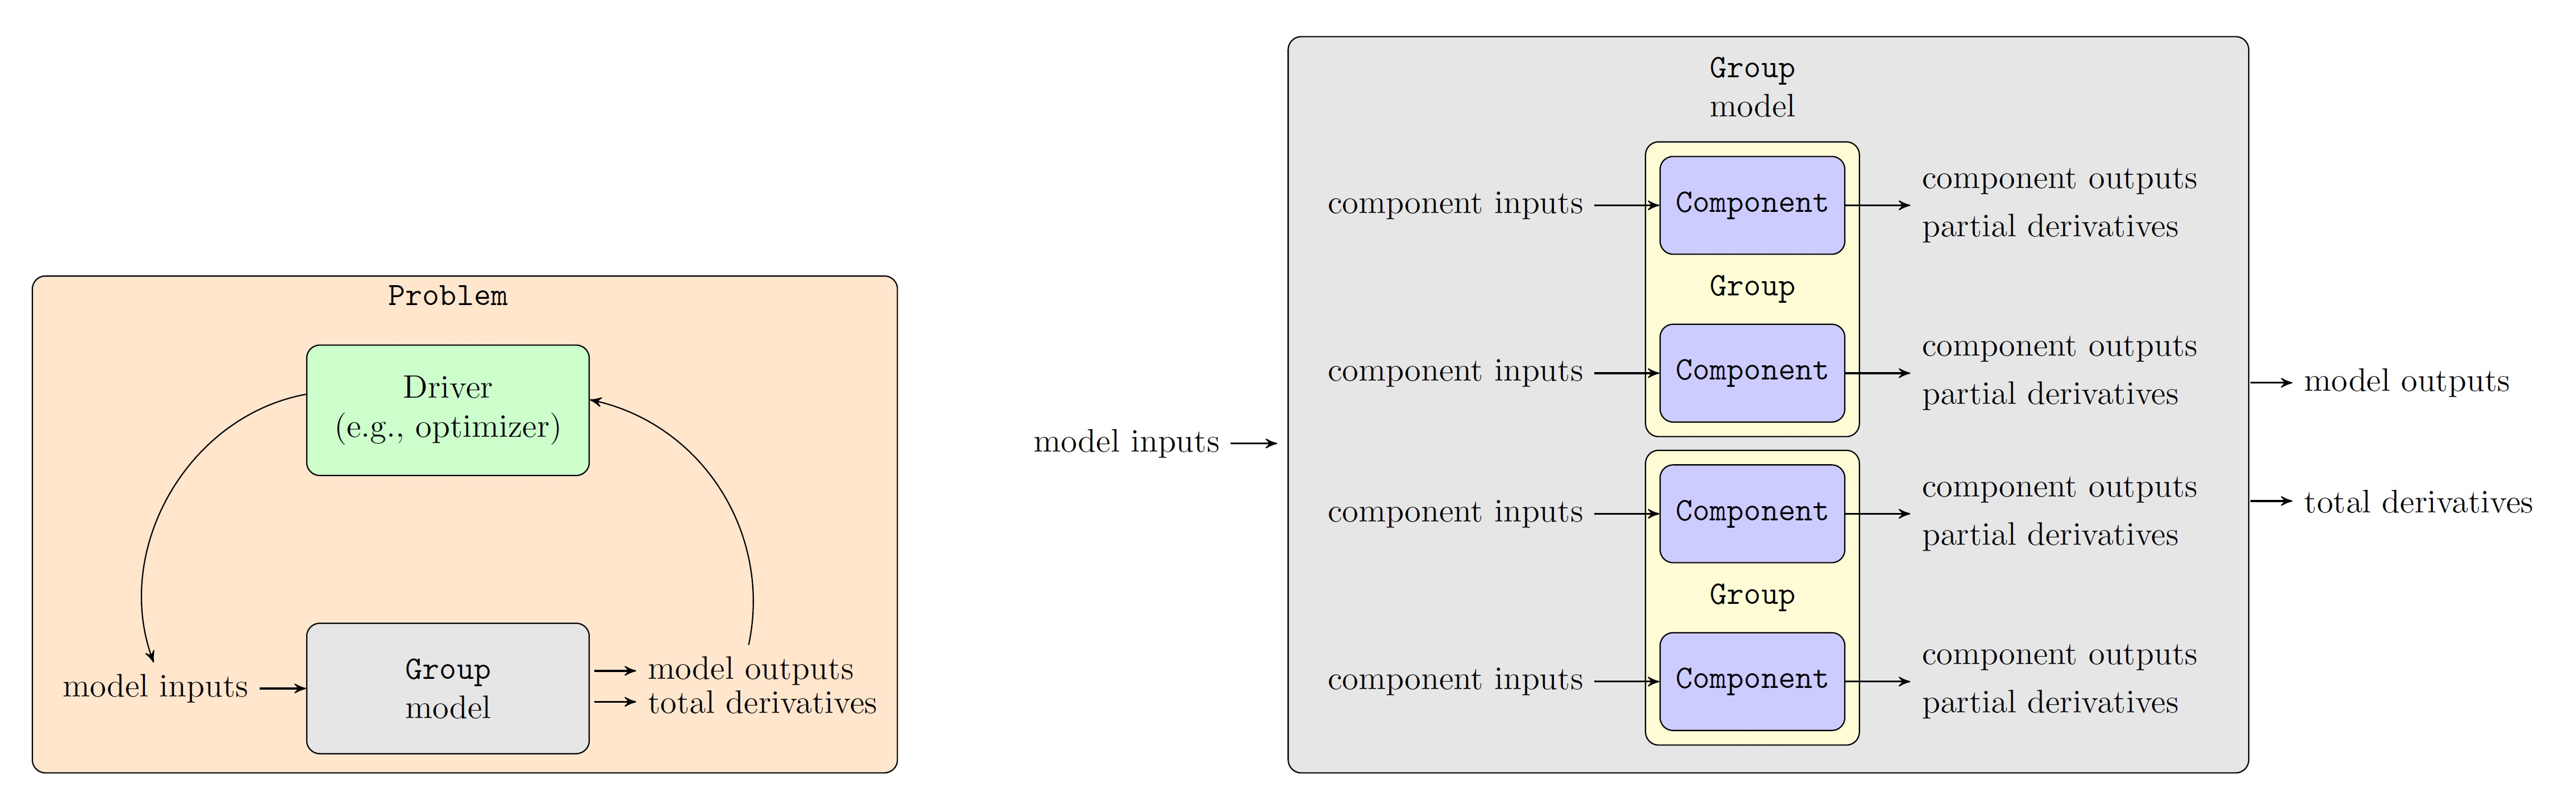
\includegraphics[keepaspectratio, width=\textwidth]{images/chap2/omdao_comp_relation.jpg}
	\caption{Relations between the OpenMDAO four basic classes: \texttt{Component, Group, Driver} and \texttt{Problem}~\cite{bib:gray_omdao}.}
	\label{fig:omdao_class_relation}
\end{figure}

Following this overview of OpenMDAO, the next step consists in detailing the integration of FAST within this optimisation platform. 

\section{The integrated plaftorm FAST and OpenMDAO}
\label{sec:chap2_fast_omdao_base}

To proceed with the integration of FAST and OpenMDAO, the disciplines must be rewritten in the OpenMDAO language, using components and groups.
For clarity, from now on the original version of FAST is referred as ``original version'' meanwhile the new one within the OpenMDAO platform is referred as ``integrated version''. 
One important difference is that under OpenMDAO, the integrated version carries out aircraft optimisation, starting from the same set of TLAR as the original version.
It must be noted that the optimisation can be carried out in other ways than using OpenMDAO, \textit{i.e.} using the gradient-free algorithms available in the \texttt{SciPy} library, or a global algorithm as SEGOMOE, jointly developed by ONERA and ISAE-Supaero~\cite{bib:bartoli_sego}.
These solutions are more intuitive and in some way simpler to implement than the complete OpenMDAO process. 
In this Ph.D., the choice has been to go with the recoding in OpenMDAO because of its various advantages, especially when dealing with derivatives, as seen from the description of previous section and the works that use OpenMDAO~\cite{bib:gray_omdao}. 
The use of derivatives has a major interest because the high efficiency of gradient-based methods, remarked also in Fig.~\ref{fig:gradbas_vs_gradfree}. 

For this reason it has been chosen to develop the integrated version of FAST considering derivatives information for aircraft optimisation.
This choice led to an imporant set-up time dedicated in the recoding of FAST under the OpenMDAO language. 
Because of this fully recoding, it has been decided to move from Python 2.7 to Python 3.7, which is a more recent and stable Python version. 

The starting point is then to convert all the disciplines as they are into \texttt{ExplicitComponent} or \texttt{ImplicitComponent}, according to their nature. 
Derivatives can be then computed with finite difference method. 
However, this is not the most efficient choice: except for some specific modules that call XFoil or OpenVSP, FAST is based on mathematical expressions: it is possible to have analytic derivatives, better in terms of required iterations (see again Fig.~\ref{fig:gradbas_vs_gradfree}). 
To facilitate their computation, each discipline has then been broken into small components, basically one \texttt{Component} instance (explicit or implicit) for each equation; subsequently all these elements have been regrouped again to form groups, each group representing a discipline, in agreement with the schema of Fig.~\ref{fig:fast_basic}.

At this stage of the process develoment, it is necessary to choose the MDO architecture: in fact the outputs definition depends on the architecture. 
Among all the possibilities, listed in the work of Martins and Lambe~\cite{bib:martins_mdo} and reported in Appendix~\ref{app:mdo_rev}, it has been decided to proceed with a Multidisciplinary Feasible (MDF) architecture, for several reasons, detailed here after:
\begin{itemize}
	
	\item It is the most intuitive to implement in the case of FAST, since the MDA loop is already defined. Also, since a recoding is necessary for the MDA, it allows to reduce the time dedicated to this phase, because it simply requires to add an optimiser at architecture top level;
	
	\item The main drawback of the MDF is that it requires a full MDA to be solved at each iteration~\cite{bib:martins_mdo}. However, because of the low CPU time for a sizing loop, this issue is not limiting;
	
	\item It requires the minor number of outputs definitions, since consistency constraints and residuals are not required;
	
	\item In case of optimisation failure before the convergence, it ensures consistency at each iteration, that is the aircraft is always consistent, albeit it may not be feasible from a constraints point of view.
	This feature may be useful for designers, because it is still possible to establish a tradeoff with design variables even if the optimisation fails, and facilitate the correction of the starting point. 
\end{itemize}

The xDSM diagram for the integrated version is shown in Fig.~\ref{fig:fast_openmdao_basic}, where the MDA loop within the MDF architecture is clearly identified. 
The equivalent algorithm is reported in Algorithm~\ref{alg:fast_openmdao_basic}.
In this schema, the engine deck initialization is explicited in this diagram (step 1).
\begin{figure}[!h]
	\centering
	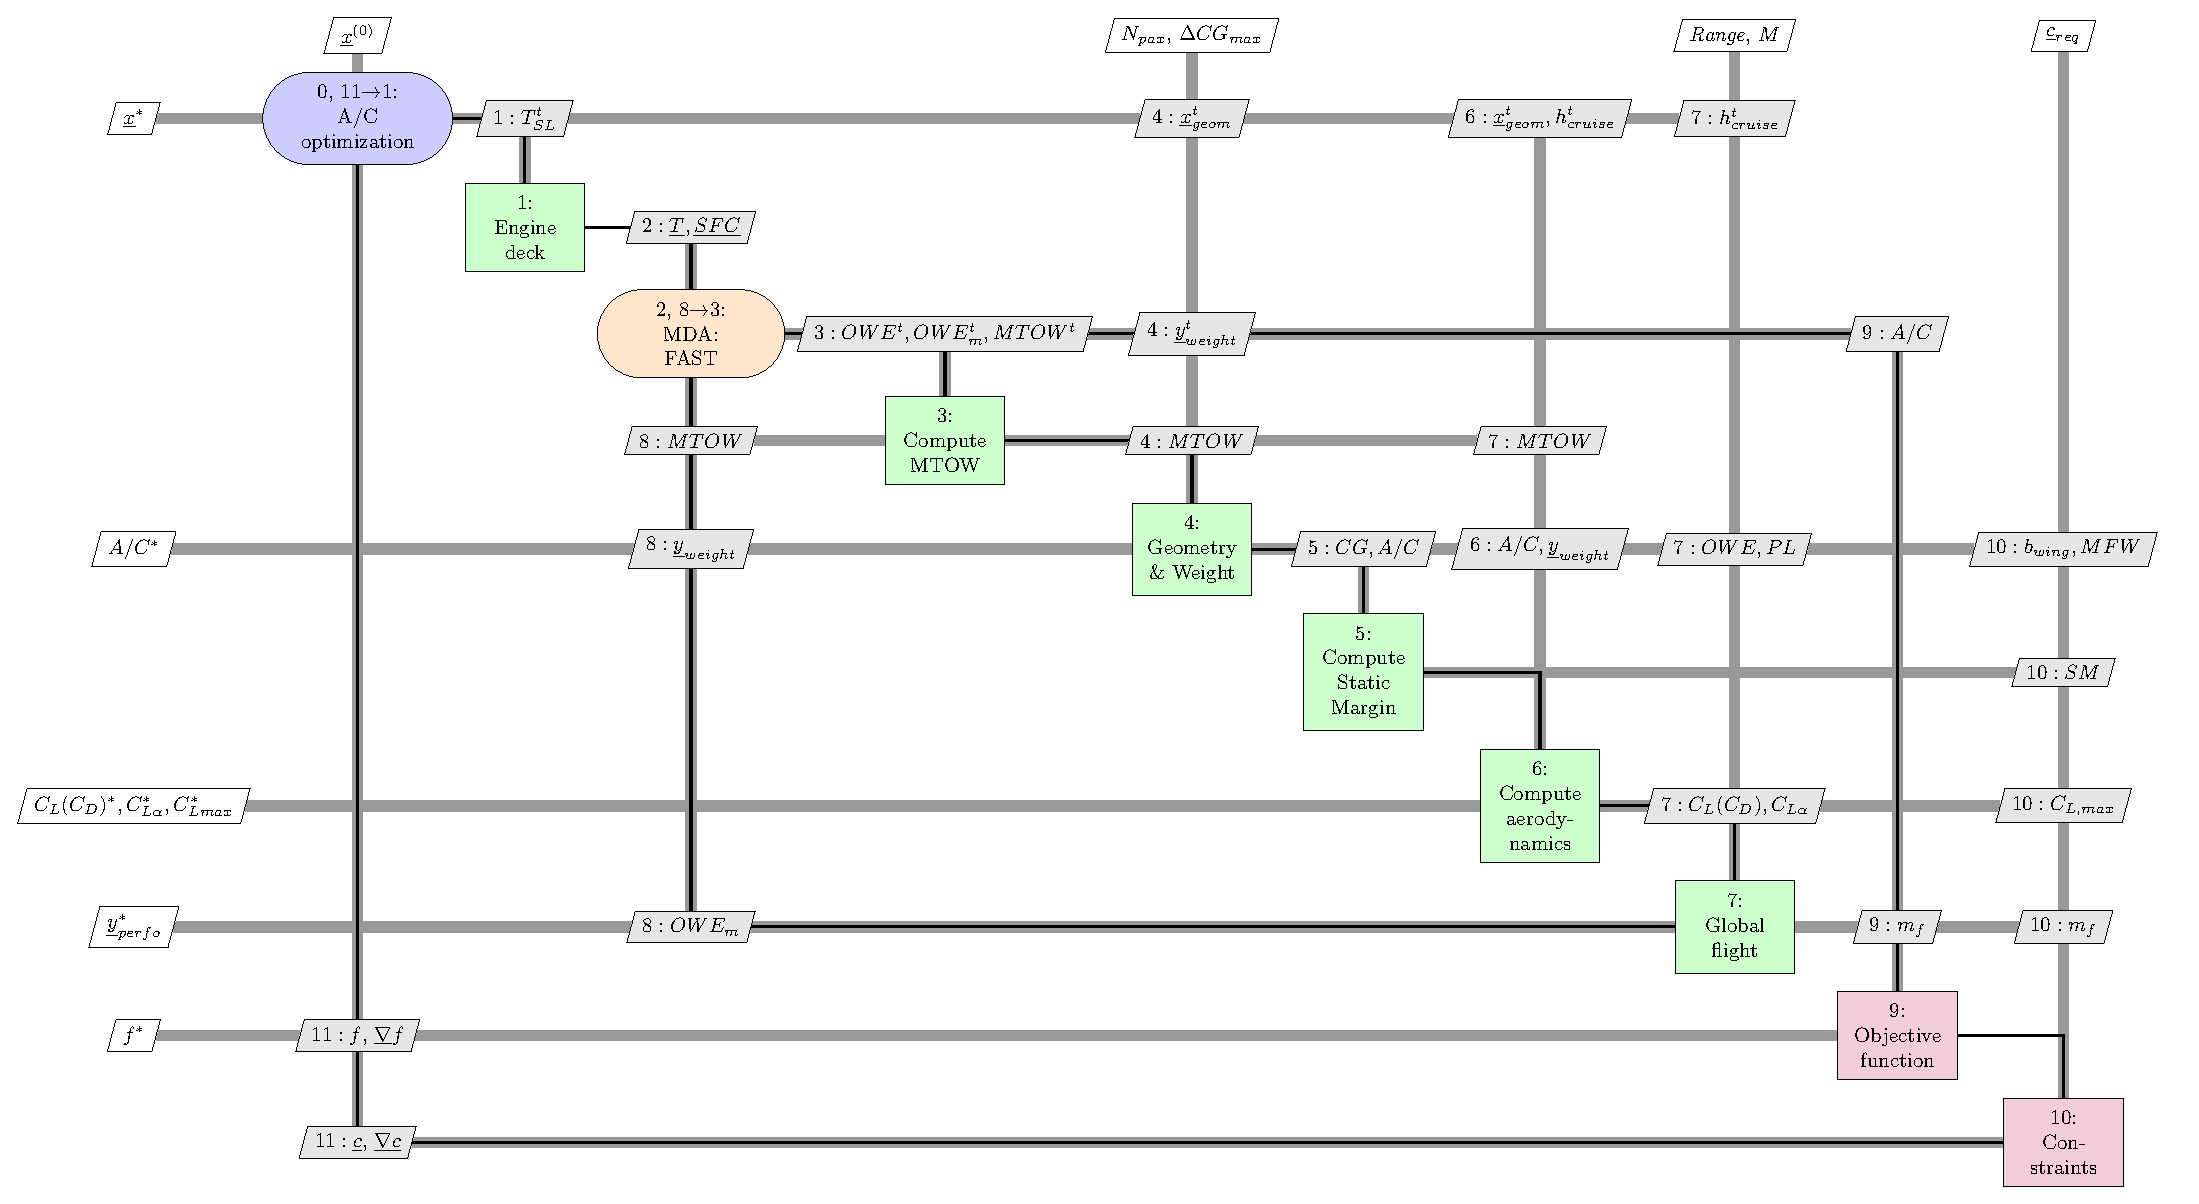
\includegraphics[keepaspectratio, width=1.3\textwidth, angle=90]{images/chap2/FAST_OpenMDAO_basic}
	\caption{xDSM diagram for the integrated version of FAST, obtained by the coupling with OpenMDAO.}
	\label{fig:fast_openmdao_basic}
\end{figure}
\begin{algorithm}[!h]
	\caption{Integrated version of FAST and OpenMDAO algorithm description, tailored to perform an optimisation of a conventional turbofan aircraft (integrated version).}
	\label{alg:fast_openmdao_basic}
	\begin{algorithmic}
		\REQUIRE Initial design parameters (TLAR), design variables initial vector $\underline{x}^{(0)}$
		\ENSURE Sized aircraft, drag polars, masses, performance, $\underline{x}^*$
		\STATE 0: Initialise the optimisation loop: initial values are read from the \texttt{xml} file.
		\REPEAT
		\STATE 1: Initialise the engine deck, using one of the models available, starting from the thrust at sea level.
		\STATE 2: Initialise the MDA (used to get a viable aircraft).
		\REPEAT
		\STATE 3: Compute MTOW.
		\STATE 4: Compute the aircraft geometry and perform the mass breakdown, to estimate weight of all components.
		\STATE 5: Compute the static margin, to check later on if the stability constraint is satisfied or not.
		\STATE 6: Aerodynamics calculation, based on the same equations of the original version.
		\STATE 7: Compute the aircraft performance.
		\STATE 8: Check the convergence. The driving parameter is the MTOW, when the error is lower than the tolerance, convergence is reached.
		\UNTIL {$8 \rightarrow 3$: MDA has converged}
		\STATE 9: Evaluate the objective function. If a gradient based solver is used, this analysis computes also derivatives.
		\STATE 10: Evaluate the design constraints. If a gradient based solver is used, this analysis computes also the derivatives of each constraint.
		\STATE 11: Check if the optimisation has converged. If not, this analysis updates $\underline{x}$ for the next iteration.
		\UNTIL {$11 \rightarrow 1$: MDO has converged}
	\end{algorithmic}
\end{algorithm}
The \texttt{xml} file is still used as I/O, but since the parameters need to be defined in OpenMDAO language, the meta-model GAMME is not used anymore. 
Instead, the dictionary is defined in Python, then an explicit component reads the \texttt{xml} and saves the values in the OpenMDAO format. 

Another consideration is that the optimisation must be ``fully opened'', in the sense that any of the chosen design variables must be constrained within a component, but it must be free to vary. 
The clearest example of this concept is the case of the wing area: in Sec.~\ref{subsubsec:chap2_fast_geom} it has been said that two values of wing area are computed, using Eq.~\eqref{eq:wing_approach_condition} and Eq.~\eqref{eq:wing_fuel_condition}, and then the maximum between the two is considered. 
In this way the design space for the wing area is limited to just two values, one for each condition to satisfy, where in real wing area can assume all the values included in an acceptable domain~\cite{bib:roskam_partI}. 
It may be that the optimal value for wing area is not one of the two explored, but another one contained in the design space.  
At the root of the optimisation logic, instead, there is the idea to define a design space exploration for each design variable.
Variables are then free to assume any value contained in its design space, it is up to the optimiser to find the optimal value that satisfies the design constraints. 

In the example of the wing area, with this logic Eq.~\eqref{eq:wing_approach_condition} and Eq.~\eqref{eq:wing_fuel_condition} are rewritten as inequalities:
\begin{equation}
	\label{eq:wing_constraint}
	\left\{\begin{array}{l}
			C_{L_{\max}} \geq \frac{m_{L}g}{\frac{1}{2}\rho V^2 S_{w}} \\
			224 S_{w}^{1.5}AR^{-0.4}\left[0.6\left(\frac{t}{c}\right)_{root}+0.4\left(\frac{t}{c}\right)_{tip}\right]+1570 \geq m_f
		\end{array}\right.
\end{equation}
Afterwards, the set of Eq.~\eqref{eq:wing_constraint} are added as design constraints, in order to let the wing area exploits all the possible values and find the optimal one that satisfies the conditions. 
The same approach applies also to the horizontal and vertical tails surface, as well as the wing position and the cruise altitude. 
In short, all the design rules that were hard coded in the original FAST, are now opened and threated as design constraints in an optimisation logic. 

As a result, the integrated version features less iterative loops than the original one: specifically the geometry module does not exhibit anymore a double loop, and concerning the performance calculations, the process does not need to iterate to find the cruise altitude. 
This can be also seen in Fig.~\ref{fig:fast_openmdao_basic_geom}, which shows the xDSM diagram for the new geometry module. 
It is clear that now the wing position is an input that serves for the SM calculation; the optimal value is chosen to minimize the objective function and to respect the SM constraints. 
\begin{figure}[!h]
	\centering
	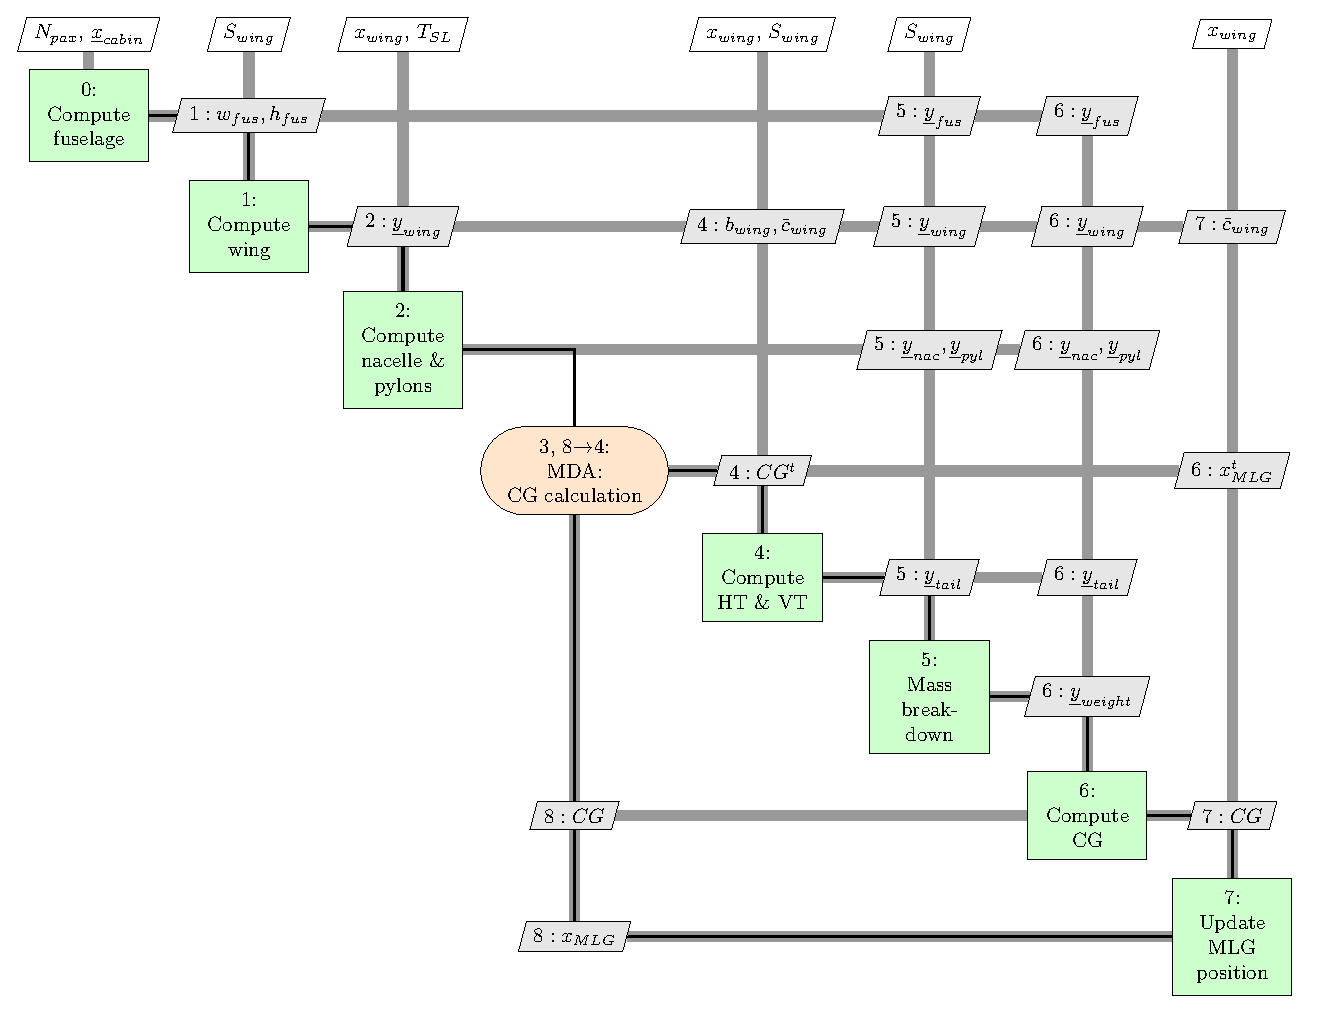
\includegraphics[keepaspectratio, width=\textwidth]{images/chap2/FAST_OpenMDAO_basic_geom}
	\caption{xDSM diagram for the geometry module of integrated version FAST and OpenMDAO.}
	\label{fig:fast_openmdao_basic_geom}
\end{figure}

Also, to fully open the problem, it has been decided to remove all the relationships between geometrical variables. 
As said in Sec.~\ref{subsubsec:chap2_fast_geom}, in fact, a lot of geometrical parameters, like the sweep of the tails, are related to the main wing parameters through statistical equations. 
From a design point of view, there are no reasons to keep these relations.
Thus and then all these parameters have been added as design variables, resulting in a larger design space exploration.

Regarding the performance analysis, beside the absence of the iterative loop to find the cruise altitude, the module is now more efficient because each mission segment has become an explicit component. 
This enables the possibility to recode the mission simulation in order to remove the issue found in the calling of descent function during the cruise leg. 
The integrated version just requires an initial guess of the distance to travel in cruise. 
Then, this value is iteratively changed until the total distance travelled for climb, cruise and descent is equals to the required range. 
With this modification, the descent component is called less than 10 times over a mission.
Compared to the hundred of times of original version that accounted for most of the computational cost, this change contributed strongly to the efficiency improvement of the process, with a reduction in time estimated in 5-10 minutes, as remarked at the end of Sec.~\ref{subsubsec:chap2_fast_perfo}. 

To consider certification specifications, the prescribed values reported in Table~\ref{tab:ccm_rules} are directly computed at the flight point of interest, since the CCM can not be used directly, having being coded using GAMME. 
However, the two formulations are totally equivalent. 
The certification conditions are then defined as design constraints, in order to let the optimiser find the optimal set of design variables that minimize the objective function, satisfying the CATPOL and CS-25 rules. 

Other minor considerations are related to the numerical schemes.
In the original version, for each iterative loop, the fixed point method was used.
In the integrated version it is possible to choose between a large variety of methods, available in OpenMDAO (like the Gauss-Seidel or the Krylov methods).
Also, robustness is increased: the original version needed to initialise the starting point because otherwise there was the risk to not get 
any results. 
OpenMDAO, instead, does not present any issue related to the choice of initial point; convergence is always ensured even with a bad choice of the initial point. 
Of course, if $\underline{x}^{(0)}$ is well chosen, the convergence is faster as the algorithm requires less iterations.

One of the possible risk of using OpenMDAO, from a user point of view, is the choice of a proper numerical scheme for convergence. 
In fact, a good choice can accelerate the convergence, but a background on numerical computation is needed~\cite{bib:leveque_partial_equation}. 
In OpenMDAO it is possible to directly solve the problem using a direct solver: it represents the easiest way since it always ensures the convergence.
On the other side it is costly since it requires a full matrix inversion~\cite{bib:gray_omdao}. 
However, starting by the v2.4, sparse matrices have been added to help the calculation. 
This results that a direct solver is efficient as a numerical scheme, which is an added feature for users. 
Finally, always related to robustness, it is worthy to note that thanks to the absence of convergence problems, the final tolerance in the integrated version is reduced of 3 orders of magnitude, from $10^{-3}$ to $10^{-6}$, resulting in more accurate results.

Despite these advantages, the integrated version presents a relevant drawback: in fact, there are more than 200 components to facilitate analytic gradient computation, compared to the 19 classes of the original one, making the code not user friendly to modifications by a new user, neither easy to understand and to use.
Also, due to the way the process is built, it is no more possible to use the code only for sizing, since parameters as wing area, wing position and so on are now design variables subject to design constraints.
In OpenMDAO, design constraints are not activated when a simple run is carried out, but they act only in an optimisation simulation. 

Also, in some cases it may be of interest to perform multiobjective optimisation, but OpenMDAO is limited to single objective problems when dealing with derivatives; from v2.4 it allows the use of NSGA-II, a genetic algorithm for multiobjective optimisation~\cite{bib:nsga2}, but it is gradient-free and thus requires long computational time. 
However, this issue can be handled with the definition of weighted functions~\cite{bib:chircop, bib:giagkiozis} or the development of specific algorithms~\cite{bib:desideri}. 
In Sec.~\ref{subsubsec:chap3_hybrid_pareto} and Sec.~\ref{subsec:chap4_bwb_pareto} examples are provided, in relations with the optimisation of the hybrid TAW and the BWB with DEP. 

The next paragraph states the optimisation problem, identifing the design variables as well as the constraints, and reports some results on the A320 CERAS validation case and a set of baseline aircraft.
These configurations will be use later on to assess performance of conventional configurations. 

\subsection{Optimisation of a turbofan aircraft with FAST under OpenMDAO}
\label{subsec:chap2_a320_optim_exploration}

\subsubsection{Problem formulation}
\label{subsubsec:chap2_a320_optim_prob_formulation}
This section presents an application of the new framework, built on the integration of FAST within OpenMDAO. 
At first, the problem must be defined: the main interest, for a civil transport aircraft, is to reduce the fuel consumption $m_f$.
This parameter becomes the objective function; all the geometrical inputs are now design variables. 
Also the cruise altitude and the thrust at sea level belongs to the design variables vector: the first is added because, in agreement with the original version, it is desired to have the aircraft always starting the cruise at the optimal altitude.
The second parameter instead allows to resize the engine according to thrust requirements. 
Finally, design constraint must be added. 
They need to ensure the feasibility of the concept, and also to comply with airport specification, top level requirements as well as certification (see Table~\ref{tab:ccm_rules}). 
The various constraints are listed below, with details to better explain the OAD problem. 
\begin{itemize}
	\item The wing has to carry all the fuel needed ($\Delta m_f = \textrm{MFW}-m_f\geq0$, being MFW the maximum fuel weight) and match the approach condition ($\Delta C_{L_{ldg}}=C_{L_{\max}}-C_{L_{app}}\geq0$).
	
	\item The horizontal tail is sized to obtain rotational performance at takeoff: the longitudinal momentum balance has to be larger than zero (zero at limit) for a given maximum center of gravity variation. This condition is defined by imposing that the total momentum is lower than zero $\Delta\mathcal{M}_{takeoff}\leq0$.
	
	\item The vertical tail is sized to have lateral stability in cruise: $S_{VT}$ has to ensure that the fuselage yaw moment is counterbalanced by the vertical tail yaw moment. 
	In mathematical symbols it can be written as $\Delta\mathcal{N}_{cruise}\geq0$, being $\mathcal{N}$ the yaw moment.
	
	\item The static margin SM has to be included between the 5\% and 10\% of the mean aerodynamics chord, in agreement with Eq.~\eqref{eq:static_margin_limits}. This condition determines the wing position $x_w$, which is placed to have SM in the required range.
	
	\item Wing span $b_w$ and takeoff field length TOFL are limited by aerodrome constraints for a medium range aircraft, in agreement with ICAO rules~\cite{bib:debarros, bib:icao}.
	
	\item The lift coefficient at the top of climb has to be equal to the value that maximizes the lift to drag ratio, to fly at the best altitude; in other words $\Delta C_{L_{toc}}=C_{L_{toc}}-C_{L_{opt}}=0$.
	
	\item The CATPOL~\cite{bib:catpol} and CS-25~\cite{bib:cs25} specifications must be satisfied as given in Table~\ref{tab:ccm_rules}. 
	In total, there are 6 constraints taken from the CCM; to simplify the process, these conditions have been collected in a single vector $$\underline{c}_{CCM}=[V_{z_{toc}}-300, V_{z_{tod}}-300, \gamma_{\%_{119a}}-3.2, \gamma_{\%_{121a}}, \gamma_{\%_{121b}}-2.4, \gamma_{\%_{121c}}-1.2, \gamma_{\%_{121d}}-2.1]$$ which must be greater than 0. 
\end{itemize}

With these notations, the problem formulation can be finally written: it is reported in Table~\ref{tab:a320_base_problem_optimisation_definition}, following the MDO community standard (see \textit{i.e.} the work of Jasa et al.~\cite{bib:jasa_topology}).
For each design variable, lower and upper bounds are defined, and this results in prescribing a design space. 
Limits are chosen recalling data on a large set of commercial single-aisle aircraft~\cite{bib:roskam_partII}. 
The size of the problem is 13, with 1 equality and 12 inequalities design constraints. 
\begin{table}[h!]
	\centering
	\begin{tabular}{l l r r r r l}
		\hline
		\textbf{Category} & \textbf{Name} & \textbf{Size} & \textbf{Lower} & \textbf{Upper} & \textbf{Equals} & \textbf{Units} \\
		\hline
		Objective & $m_f$ & 1 & -- & -- & -- & \si{\kilogram} \\
		\hline
		Variables & $S_w$ & 1 & \num{100} & \num{150} & -- & \si{\square\meter} \\
		& $x_w$ & 1 & \num{15} & \num{20} & -- & \si{\meter} \\
		& $AR_{w}$ & 1 & \num{8} & \num{12} & -- & -- \\
		& $\lambda_{w}$ & 1 & \num{0.2} & \num{0.6} & -- & -- \\
		& $\Lambda_{25_{w}}$ & 1 & \num{20} & \num{45} & -- & \si{\deg} \\
		& $\left(\frac{t}{c}\right)_w$ & 1 & \num{0.1} & \num{0.15} & -- & -- \\
		& $S_{HT}$ & 1 & \num{20} & \num{60} & -- & \si{\square\meter} \\
		& $AR_{HT}$ & 1 & \num{2} & \num{5} & -- & -- \\
		& $\lambda_{HT}$ & 1 & \num{0.2} & \num{0.6} & -- & -- \\
		& $\Lambda_{25_{HT}}$ & 1 & \num{20} & \num{45} & -- & \si{\deg} \\
		& $\left(\frac{t}{c}\right)_{HT}$ & 1 & \num{0.1} & \num{0.15} & -- & -- \\
		& $S_{VT}$ & 1 & \num{15} & \num{50} & -- & \si{\square\meter} \\
		& $AR_{VT}$ & 1 & \num{1} & \num{2.5} & -- & -- \\
		& $\lambda_{VT}$ & 1 & \num{0.3} & \num{1.0} & -- & -- \\
		& $\Lambda_{25_{VT}}$ & 1 & \num{25} & \num{55} & -- & \si{\deg} \\
		& $\left(\frac{t}{c}\right)_{VT}$ & 1 & \num{0.13} & \num{0.18} & -- & -- \\
		& $T_{SL}$ & 1 & \num{90} & \num{130} & -- & \si{\kilo\newton} \\
		& $h_{toc}$ & 1 & \num{30000} & \num{40000} & -- & ft \\
		& \textbf{Total} & 18 & & & & \\
		\hline
		Constraints & $\Delta m_{f}$ & 1 & 0 & -- & -- & \si{\kilogram} \\
		& $\Delta C_{L_{app}}$ & 1 & 0 & -- & -- & -- \\
		& $b_w$ & 1 & -- & \num{36} & -- & \si{\meter} \\
		& $\mathcal{M}_{takeoff}$ & 1 & -- & \num{0} & -- & \si{\newton\meter}  \\
		& $\Delta \mathcal{N}_{cruise}$ & 1 & \num{0} & -- & -- & \si{\newton\meter} \\
		& TOFL & 1 & -- & \num{2200} & -- & \si{\meter} \\
		& $\Delta C_{L_{toc}}$ & 1 & -- & -- & 0 & -- \\
		& SM & 1 & \num{0.05} & \num{0.10} & -- & -- \\
		& $\underline{c}_{CCM}$ & 5 & \num{0} & -- & -- & \% \\
		& \textbf{Total} & 13 & & & & \\
		\hline    	
	\end{tabular} 
	\caption{Optimisation problem definition for the A320 CERAS case. Variables' limits come from literature review on single aisle type aircraft~\cite{bib:roskam_partII}.}
	\label{tab:a320_base_problem_optimisation_definition}
\end{table}

\subsubsection{Test case: A320 CERAS aircraft}
\label{subsubsec:chap2_a320_optim_ceras}

The first test case to be analysed is the optimisation of the A320 CERAS aircraft, already studied with the original version of FAST in Section~\ref{subsec:chap2_fast_test_case}, associated to TLAR reported in Table~\ref{tab:fast_base_tlar}. 
One issue regarding gradient-based methods is that the optimum point $\underline{x}^*$ can be a local minimum~\cite{bib:martins_mdo}.
To increase the likelihood of convergence to the global optimum, a multistart check is performed, with 10 different initial vectors $\underline{x}^{(0)}$.
If $\underline{x}^*$ does not depend on initial value, then it is assumed as global minimum; otherwise it is reasonable to consider that the global minimum is within the obtained solutions.
The 10 starting points are chosen through the creation of a Latin hypercube sampling LHS~\cite{bib:sacks}. 

Table~\ref{tab:optimisation_setup} reports the set-up that is used: the optimisation solver is SNOPT~\cite{bib:snopt}, a sequential least squares programming algorithm, that derives from SLSQP algorithm~\cite{bib:slsqp}, and included in the \texttt{pyOptSparse} library. 
It has been chosen because it is one of the most efficient gradient based algorithm (see also Fig.~\ref{fig:gradbas_vs_gradfree}), that supports both inequalities and equalities constraints~\cite{bib:snopt}. 
Linear and non-linear solver are respectively the Gauss--Seidel and the direct solver.
The utilisation of direct solver in place of a numerical method is justified by the consideration done in Sec.~\ref{sec:chap2_openmdao_overview}.
Starting from OpenMDAO 2.4, the implementation of sparse matrices makes the two methods comparable in terms of performance. 
Direct solver facilitates the setting, since it does not require the definition of pre-conditioner or similar options, and thus it is considered in this optimisation problem. 
Tolerance, both for MDA and MDO, is $10^{-6}$ as default value. 
\begin{table}[!h]
	\centering
	\begin{tabular}{l r}
		\hline
		\textbf{optimisation solver} & SNOPT \\
		\textbf{Linear solver} & Linear Gauss-Seidel \\
		\textbf{Non linear solver} & Direct solver \\
		\textbf{MDA tolerance} & $10^{-6}$ \\
		\textbf{optimisation tolerance} & $10^{-6}$ \\
		\hline
	\end{tabular}
	\caption{Set-up for the A320 CERAS optimisation problem, using gradient based method.}
	\label{tab:optimisation_setup}
\end{table}

Table~\ref{tab:a320_base_optim_comparison} reports a comparison between the quantities of interest for the considered test case, both for baseline and optimised aircraft, meanwhile Table~\ref{tab:a320_base_optim_dv} reports the design variables values.
The geometrical input parameters for the baseline are the same of Table~\ref{tab:fast_base_geom_inp}.
Note that most of the variables of Table~\ref{tab:a320_base_optim_dv} are computed within the original version with statistical equations, meanwhile in the integrated version they are free to vary within their specified range.
The mission profile is defined by using values of Table~\ref{tab:fast_base_thrust_rate_entry} for thrust setting. 
\begin{table}[!h]
	\centering
	\begin{tabular}{l l c c}
		\hline
		& & \textbf{Baseline} & \textbf{optimised} \\
		\hline
		\textbf{MTOW} & [\si{\tonne}] & 74.2 & 73.7 \\
		\textbf{OWE} & [\si{\tonne}] & 42.2 & 42.4 \\
		\textbf{Wing area} & [\si{\square\meter}] & 122.74 & 123.38 \\
		\textbf{Max. LoD} & & 15.9 & 17.1 \\
		\textbf{Static margin} & & 0.10 & 0.05 \\
		\textbf{Fuel mission} & [\si{\tonne}] & 18.7 & 17.1 \\
		\hline
		\textbf{CAT.POL.A.410(a)-1} & [ft/min] & 964.69 & 913.17 \\
		\textbf{CAT.POL.A.410(a)-2} & [ft/min] & 1031.82 & 663.85 \\
		\textbf{CS-25.119(a)} & [\%] & 19.46 & 17.82 \\
		\textbf{CS-25.121(a)} & [\%] & 1.61 & 2.01 \\
		\textbf{CS-25.121(b)} & [\%] & 3.43 & 2.47 \\
		\textbf{CS-25.121(c)} & [\%] & 5.56 & 5.30 \\
		\textbf{CS-25.121(d)} & [\%] & 7.19 & 6.78 \\
		\hline
	\end{tabular}
	\caption{Comparison between quantities of interest for the baseline and the optimised aircraft, A320 CERAS test case. Top level requirements are reported in Table~\ref{tab:fast_base_tlar}.}
	\label{tab:a320_base_optim_comparison}
\end{table}

\begin{table}[!h]
	\centering
	\begin{tabular}{l l c c}
		\hline
		& & \textbf{Baseline} & \textbf{optimised} \\
		\hline
		$S_w$ & [\si{\square\meter}] & 122.74 & 123.38  \\
		$x_w$ & [\si{\meter}] & \num{16.61} & \num{15.94}  \\
		$AR_{w}$ & & 9.5 & 10.6 \\
		$\lambda_{w}$ & & 0.38 & 0.33 \\
		$\Lambda_{25,w}$ & [\si{\deg}] & 25 & 23.4  \\
		$\left(\frac{t}{c}\right)_w$ & & 0.128 & 0.117\\
		$S_{HT}$ & [\si{\square\meter}] & 33.28 & 29.32  \\
		$AR_{HT}$ & & 43.28 & 3.74  \\
		$\lambda_{HT}$ & & 0.4 & 0.2  \\
		$\Lambda_{25,HT}$ & [\si{\deg}] & 28 & 32.14  \\
		$\left(\frac{t}{c}\right)_{HT}$ & & 0.1 & 0.1 \\
		$S_{VT}$ & [\si{\square\meter}] & 29.53 & 26.23  \\
		$AR_{VT}$ & & 1.74 & 1.2 \\
		$\lambda_{VT}$ & & 0.3 & 0.3  \\
		$\Lambda_{25,VT}$ & & [\si{\deg}] 35 & 35  \\
		$\left(\frac{t}{c}\right)_{VT}$ & & 0.1 & 0.1  \\
		$T_{SL}$ & [\si{\kilo\newton}] & 117.8 & 108.2  \\
		$h_{toc}$ & [ft] & 34000 & 33248  \\
		\hline
	\end{tabular}
	\caption{Comparison between design variables for the A320 CERAS test case baseline and optimised. Geometric inputs for the baseline are in agreement with Table~\ref{tab:fast_base_geom_inp}.}
	\label{tab:a320_base_optim_dv}
\end{table}

The first point to note is that the aspect ratio is increased. 
The optimiser finds that the optimal path goes towards a larger wing, that uses all the span possible (36~\si{\meter}).
As a result, the maximum lift-to-drag ratio is increased of about 8\%.
Also the OWE is slightly higher, because of bigger wing. 
However, the aerodynamics benefits overcome the penalties in weight, and the fuel consumption is reduced of about 9\%. 
This also results in a reduced MTOW. 
Another difference lies in the static margin: the original version, indeed, was coded in order that the internal loop stops the first time the static margin stays within the range of 5-10\%. 
This means that, if the initial wing position is backwarded, the SM achieved is always 0.10. 
In the integrated version, instead, the optimiser finds the most forwarded position, in order to increase tail level arm and to reduce the tail size. 
Also, aspect ratio and sweep of the horizontal tail are optimised to move the aerodynamics center in the farest position as possible, always to advance the wing the most allowable. 

Table~\ref{tab:a320_base_optim_comparison} reports also the values achieved for the various certification constraints during the sizing loop. 
It is interesting to note that the thrust of the engine is reduced while complying with the CS-25.121(b).
The reduction in thrust contributes to the increase in maximum lift-to-drag ratio too, since the engine wetted area is reduced. 

These results show that the problem is well-posed, and that the optimiser goes towards the best solution. 
Also, it is verified that with the 10 multistart approach, there are no local minima. 
In order to understand the presence of more minima, the objective function value and the norm of constraints are evaluated.
Considering the constraint written in the form $\underline{c}=[g_i\left(\underline{x}\right)-a_i]\leq0$, with $i=1,\cdots,N$, this last quantity is defined as: 
\begin{equation}
	\label{eq:norm_constraint}
	\Vert \underline c \Vert = \sum_{i=0}^{N}\vert g_i\left(\underline{x}\right)-a_i \vert
\end{equation}
where 
\begin{equation}
	\label{eq:sum_violation_constraint}
	\vert g_i\left(\underline{x}\right)-a_i \vert = \left\{
	\begin{array}{l l}
		0 & g_i\left(\underline{x}\right) \leq a_i + \epsilon \\
		g_i\left(\underline{x}\right)-a_i & \textrm{otherwise}
	\end{array} \right.
\end{equation}
with $\epsilon$ being the tolerance.
In other word, if a constraint is violated the norm is computed as the difference with respect to the minimum value, otherwise it is set to zero. 
As a consequence, a feasible point has the norm of the constraints equals to zero. 

Table~\ref{tab:a320_base_optim_multipoint_result} reports the final objective function $f^\star$ and the norm of constraints for the 10 runs: all the points are feasible, and no local minima are detected, since the maximum difference among the 10 $f^\star$ is less of 0.4\%.
\begin{table}[!h]
	\centering
	\begin{tabular}{l c c c c c c c c c c}
		\cline{2-11}
		& \multicolumn{10}{c}{\textbf{Run}} \\
		\cline{2-11}
		& 1 & 2 & 3 & 4 & 5 & 6 & 7 & 8 & 9 & 10 \\
		\hline
		$f^\star$ & 17094 & 17151 & 17086 & 17092 & 17139 & 17101 & 17089 & 17128 & 17112 & 17104 \\
		$\Vert \underline c \Vert$ & 0 & 0 & 0 & 0 & 0 & 0 & 0 & 0 & 0 & 0\\
		\hline
	\end{tabular}
	\caption{Objective function and norm constraints, defined as in Eq.~\eqref{eq:sum_violation_constraint}, for the 10 optimisation runs carried out for A320 CERAS test case baseline.}
	\label{tab:a320_base_optim_multipoint_result}
\end{table}

The payload-range is also computed with the integrated process: a comparison between the baseline and the optimised aircraft is shown in Fig.~\ref{fig:a320_base_optim_pl_range}. 
Only minor differences are detected: because of the reduced MTOW, the first horizontal segment is shorter, but then better aerodynamics and larger fuel capacity make the ferry range of the aircraft higher, even if the difference is of only few nautical miles. 
\begin{figure}[!h]
	\centering
	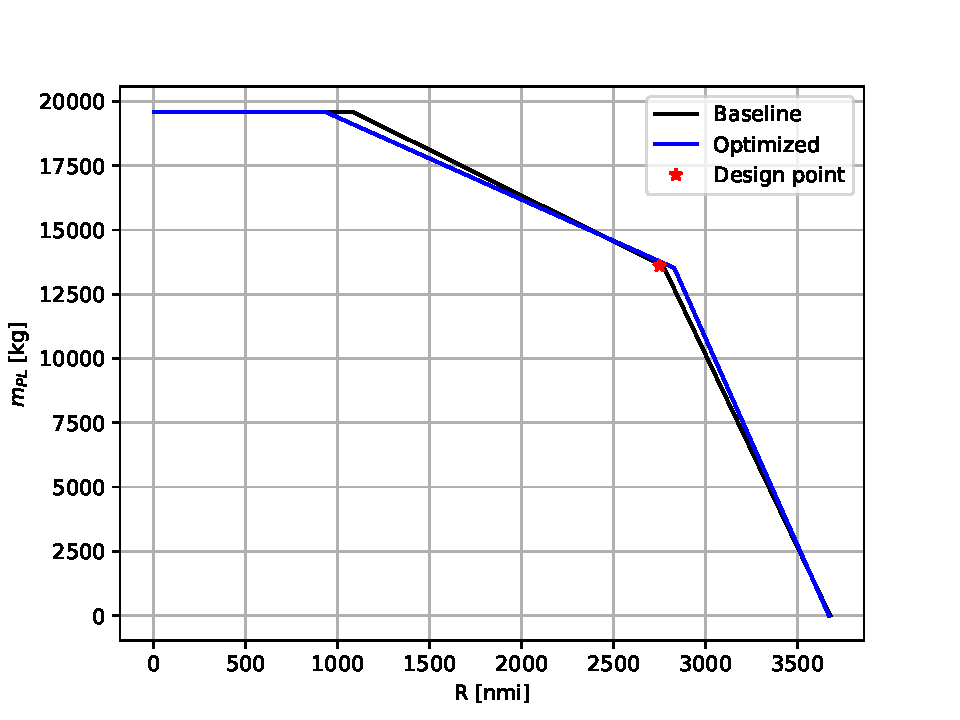
\includegraphics[keepaspectratio, width=0.6\textwidth]{images/chap2/fast_base_optim_pl_range}
	\caption{Payload-Range diagram, for the A320 CERAS test case, baseline and optimised aircraft.}
	\label{fig:a320_base_optim_pl_range}
\end{figure}

The code took about 35~\si{\minute} to reach the convergence; a total of 36 iterations, with 39 call to objective functions, have been needed to find the solution. 
The convergence history is shown in Fig.~\ref{fig:a320_optim_conv_history}. 
The algorithm finds very soon the minimum: indeed after 20 iterations, variations are so small that the objective value can be assumed constant. 
Note that up to iteration 10 the objective function is smaller than the final value, but these points do not respect the full set of design constraints and are not feasible. 
\begin{figure}[!h]
	\centering
	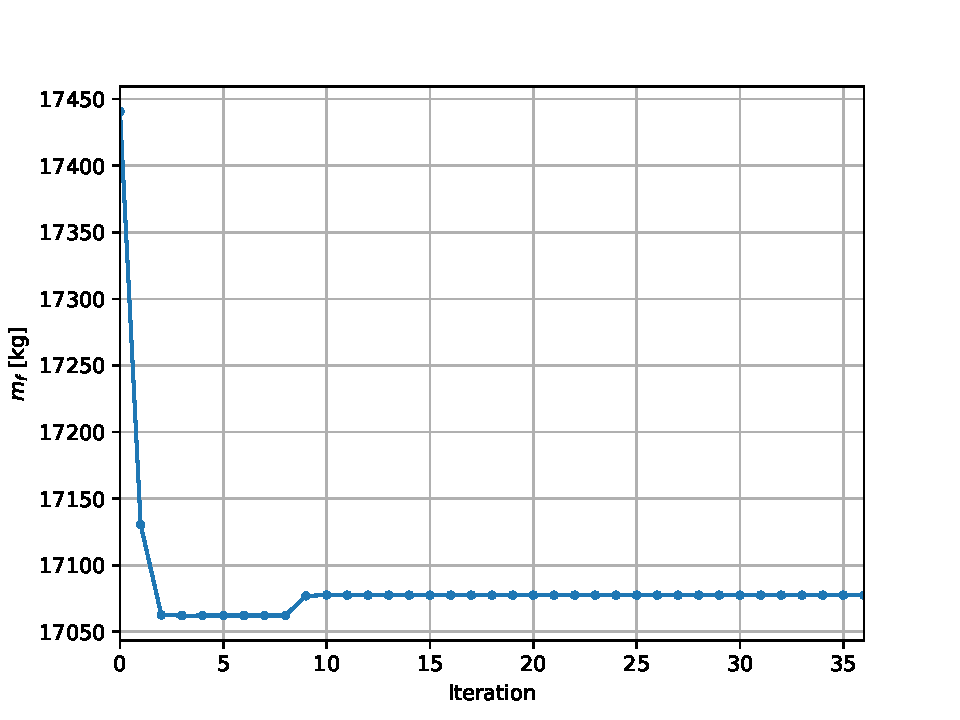
\includegraphics[keepaspectratio, width=0.6\textwidth]{images/chap2/fast_optim_conv_history}
	\caption{Convergence history for optimisation problem of A320 CERAS test case.}
	\label{fig:a320_optim_conv_history}
\end{figure}

\subsubsection{Test case: A320 CERAS resized for EIS2035}
\label{subsubsec:chap2_a320_optim_eis2035}

In this section, the integrated code is used to generate the baseline aircraft to be used as comparison for the assessment of unconventional configurations.
The technological horizon is 2035, which means that some assumptions have to be made for the mass estimation, the engine model and aerodynamics. 
The TLAR are practically the same, except for the range, that not 2750~nmi anymore. 
Its variation is instead limited from 600 to 1500~nmi.
This choice is dictated by the marketing.
According to an Airbus analysis, in fact, most of the aircraft fly in this operational range, and thus for the future can be considered to have new resized aircraft on these ranges~\cite{bib:airbus_global_market}. 
For clarity, the new TLAR are reported in Table~\ref{tab:a320_2035_tlar}. 
The mission profile is still the one of the A320 CERAS reference aircraft, presented in Table~\ref{tab:fast_base_thrust_rate_entry}. 
\begin{table}[!h]
	\centering
	\begin{tabular}{l r r}
		\hline
		Range & 600--1500 & nmi \\
		Number of passengers & 150 & \\
		Approach speed & 132 & \si{\knot} \\
		Design payload & 13608 & \si{\kilogram} \\
		\hline		
	\end{tabular}
	\caption{Top level requirements for the resized A320, considering EIS2035.}
	\label{tab:a320_2035_tlar}
\end{table} 

For the technological assumptions, the most reliable document available so far in literature is the IATA report~\cite{bib:iata, bib:iata_annex}, which states perspectives of available technologies in a 20 year period and their foreseen impact. 
Regarding the mass estimation, the use of innovative materials, like new alloys or composites, reduces the weight of the aircraft. 
The estimated impact of new technologies is reported in Table~\ref{tab:2035_mass_impact}. 
\begin{table}[!h]
	\centering
	\begin{tabular}{l c}
		\hline
		\textbf{Component} & \textbf{Impact on mass} \\
		\hline
		Wing & -10\% \\
		Fuselage & -5\% \\
		Landing gear & -15\% \\
		Pylons & -10\% \\
		Passenger seats & -60\% \\
		\hline
	\end{tabular}
	\caption{Impact of new technologies on airframe mass estimation according to IATA~\cite{bib:iata_annex}, considering EIS2035.}
	\label{tab:2035_mass_impact}
\end{table}
These estimations are not the only one available in literature, however they seem to be the more reasonable in the chosen technological horizon. 
The gains at discipline or component level have been implemented through the corrective factors technique, as described in Section~\ref{sec:chap2_fast_base_description}. 

For aerodynamics, improvements can be foreseen thanks to the introduction of different new technologies~\cite{bib:iata_annex}: 
\begin{itemize}
	\item \textbf{New winglet design}. A careful winglet design, with innovative and optimised shape, could lead to a reduction on the induced drag up to 10\%.
	
	\item \textbf{Laminarity drag coating}. The use of a film coating on the wing can reduce the roughness in order to achieve a fully laminar flow and reduce the friction coefficient up to 20\%. In practice, it is very sensitive to external condition and it is not said that the flow will be in any condition laminar.
	
	\item \textbf{Turbulent drag coating}. This technology is complementary to the previous one. A rough coating is added on the wing to induce turbulence: despite the flow results more viscous, the turbulence avoids separation and its impact on the $C_{D_{0}}$ is estimated to be of 5\%. Also, it is less sensitive to external condition than the laminarity drag coating.
	
	\item \textbf{Natural laminar flow control}. An accurate wing design can be achieved to naturally have laminar flow over the wing. In practice, this solution is unfeasible for wing with sweep angles higher than 20~\si{\degree}. 
	
	\item \textbf{Shock contol}. This technology uses a bump over the wing to control the shock wave geometry even in off-design conditions. 
	It may reduce the wave drag coefficient up to 50\%.
	
	\item \textbf{Morphing wing}. The idea at the back of this technology is to use smart materials that change the wing shape, in order to always adapt the geometry to external condition and increase the aerodynamics efficiency. 
	Its reduction on the total drag coefficient is estimated to be of about 3.2\%. 
	
	\item \textbf{Hybrid laminarity flow control (HLFC)}. In this case, laminarity is achieved throught both accurate wing design and active flow control to ingest boundary layer. Its effect on the friction coefficient is about 45-50\%. In practice the system introduces relevant penalties in weight, that may counterbalance the aerodynamics benefits. Also, its integration within the airframe is very challenging. 
\end{itemize}
For the 2035 reference aircraft, new winglet design, shock control and morphing wing are considered. 
The turbulent drag coating is also taken into in spite of the laminarity drag coating, because it is less sensitive to external condition and then more reliable. 
A natural shock control is unfeasible because of the transonic region, which requires a swept wing. 
Finally, HLFC is not considered because of limited knowledge at this stage: low maturity and penalties assessment are complex to quantify and it can introduce potential risks to the design. 

The final impacts on aerodynamics are reported in Table~\ref{tab:2035_aero_impact}.
As for the weight, variations have been implemented using corrective factors in Eq.~\eqref{eq:cd_total}. 
\begin{table}[!h]
	\centering
	\begin{tabular}{l c c}
		\hline
		\textbf{Technology} & \textbf{Parameter} & \textbf{Impact} \\
		\hline
		Winglet design & $C_{D_{i}}$ & -10\% \\
		Turbulent drag coating & $C_{D_{0}}$ & -5\% \\
		Shock control & $C_{D_{c}}$ & -50\% \\
		Morphing wing & $C_D$ & -3.2\% \\
		\hline
	\end{tabular}
	\caption{Impact of new technologies on aerodynamics according to IATA~\cite{bib:iata_annex}, considering EIS2035.}
	\label{tab:2035_aero_impact}
\end{table}

Some assumptions at engine level have also to be made. 
It is reasonable to consider that engines in the future will belong to ultra by-pass ratio category, as for the LEAP engine~\cite{bib:leap_engine}: these engines have a greater BPR, to increase the thrust generated by cold flow and consequently reduce the SFC. 
Current technology shows a maximum BPR of 11-12. 
It is foreseen that this value shall not be exceeded, to keep fan dimensions within the limits, but the engine improvements will be mainly related to a more efficient combustion process. 
To match 2035 assumptions, a BPR equals to 11 is taken into account, to have the effect of wetted areas, together with a reduction of SFC and an impact on the masses, due to a combined effect of larger engines and new materials. 

With these assumptions, it is finally possible to proceed with the sizing of a new set of A320 type aircraft, that matches the EIS2035. 
Again, the optimised aircraft is compared with some baseline, obtained with the original version using the geometrical input of Table~\ref{tab:fast_base_geom_inp}. 

The fuel consumption as a function of the design range is shown in Fig.~\ref{fig:a320_2035_optim_comp}, for the baseline and the optimised aircraft. 
For completeness, key parameters for each configuration are reported in Table~\ref{tab:a320_2035_non_optim_res} (baseline) and Table~\ref{tab:a320_2035_optim_res} (optimised). 
The optimised configuration shows a fuel saving in the order of 10-15\%; also since the slope of the curve of Fig.~\ref{fig:a320_2035_optim_comp} is lower for optimised aircraft, it can be expected that the impact will be greater on longer range. 
Same considerations done for the optimum point in Section~\ref{subsubsec:chap2_a320_optim_ceras} can be retaken here. 
Concerning certification constraints, for shorter range aircraft it is important to note that the sizing condition for the thrust is not anymore the slope at 400~ft of altitude, corresponding to CS-25.121(b), but more the CAT.POL.A.410(a)-2, which corresponds to the vertical speed reserve at the top of descent. 
This can be explained because the aircraft is more efficient, and therefore consumes less fuel. 
So the difference in weight between the beginning and the end of the cruise is reduced, and due to the higher mass it needs more thrust at the top of descent to match the needed $V_z$. 
On the other hand, condition CS-25.121(b), which was the most stringent condition in the case of Table~\ref{tab:a320_base_optim_comparison}, decreases with respect to range, so it can be expected that on longer range, where also the aircraft is lightened more because of the greater distance, it will be again the sizing condition for maximum thrust, in agreement with previous case. 
\begin{figure}[!h]
	\centering
	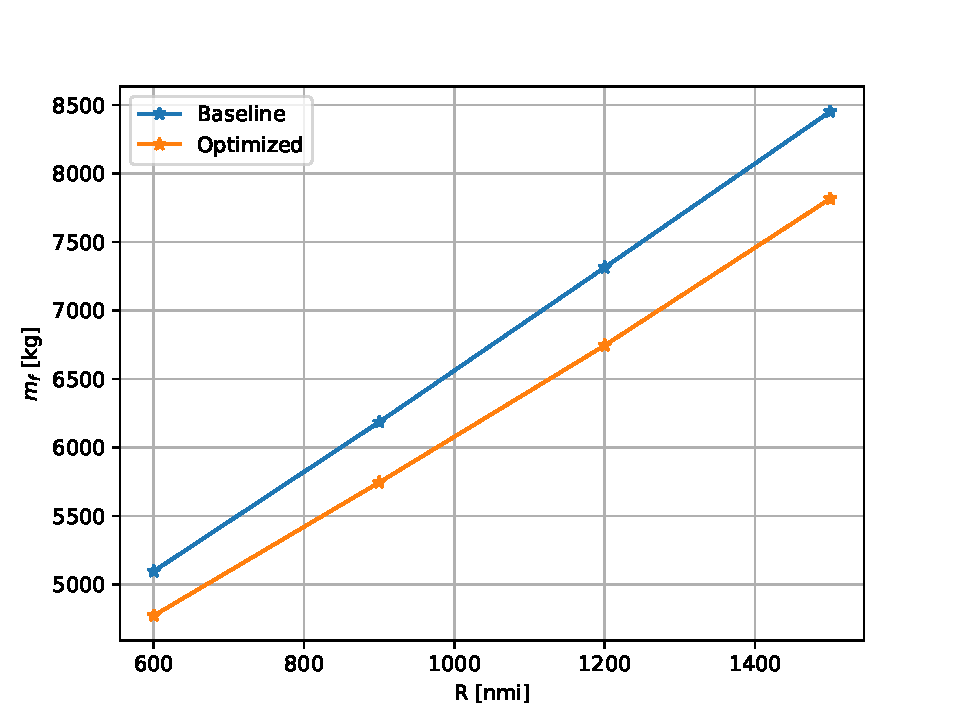
\includegraphics[keepaspectratio, width=0.6\textwidth]{images/chap2/fast_base_optim_comp}
	\caption{Fuel consumption as a function of design range for the A320 baseline and the optimised aircraft, resized to match EIS2035. TLAR are reported in Table~\ref{tab:a320_2035_tlar}. }
	\label{fig:a320_2035_optim_comp}
\end{figure}

\begin{table}[!h]
	\centering
	\begin{tabular}{l l c c c c}
		\cline{3-6}
		& & \multicolumn{4}{c}{\textbf{Range} [nmi]} \\
		& & \textbf{600} & \textbf{900} & \textbf{1200} & \textbf{1500} \\
		\hline
		\textbf{MTOW} & [\si{\tonne}] & 58.83 & 60.02 & 61.24 & 62.48 \\
		\textbf{OWE} & [\si{\tonne}] & 40.21 & 40.31 & 40.4 & 40.49  \\
		\textbf{Wing area} & [\si{\square\meter}] & 118.79 & 118.97 & 119.16 & 119.35 \\
		\textbf{Max. LoD} & & 17.44 & 17.44 & 17.43 & 17.43 \\
		\textbf{Fuel mission} & [\si{\tonne}] & 5.09 & 6.18 & 7.31 & 8.45 \\
		\hline
		\textbf{CAT.POL.A.410(a)-1} & [ft/min] & 932.18 & 929.41 & 928.88 & 927.4 \\
		\textbf{CAT.POL.A.410(a)-2} & [ft/min] & 786.4 & 780.39 & 774.13 & 767.66 \\
		\textbf{CS-25.119(a)} & [\%] & 21.98 & 21.92 & 21.87 & 21.81 \\
		\textbf{CS-25.121(a)} & [\%] & 6.01 & 5.65 & 5.31 & 4.97 \\
		\textbf{CS-25.121(b)} & [\%] & 7.94 & 7.64 & 7.28 & 6.91 \\
		\textbf{CS-25.121(c)} & [\%] & 8.84 & 8.57 & 8.29 & 8.05 \\
		\textbf{CS-25.121(d)} & [\%] & 8.8 & 8.76 & 8.72 & 8.68 \\
		\hline
	\end{tabular}
	\caption{Quantities of interest for the A320 case baseline, resized to match EIS2035 with TLAR reported in Table~\ref{tab:a320_2035_tlar} and geometrical inputs as in Table~\ref{tab:fast_base_geom_inp}.}
	\label{tab:a320_2035_non_optim_res}
\end{table}

\begin{table}[!h]
	\centering
	\begin{tabular}{l l c c c c}
		\cline{3-6}
		& & \multicolumn{4}{c}{\textbf{Range} [nmi]} \\
		& & \textbf{600} & \textbf{900} & \textbf{1200} & \textbf{1500} \\
		\hline
		\textbf{MTOW} & [\si{\tonne}] & 56.76 & 57.89 & 59.01 & 60.14 \\
		\textbf{OWE} & [\si{\tonne}] & 38.58 & 38.71 & 38.79 & 38.84  \\
		\textbf{Wing area} & [\si{\square\meter}] & 116.21 & 116.47 & 116.63 & 116.76 \\
		\textbf{Max. LoD} & & 18.47 & 18.46 & 18.45 & 18.44 \\
		\textbf{Thrust @ SL} & [\si{\kilo\newton}] & 99.5 & 100 & 100 & 99.75 \\
		\textbf{Fuel mission} & [\si{\tonne}] & 4.77 & 5.74 & 6.77 & 7.81 \\
		\hline
		\textbf{CAT.POL.A.410(a)-1} & [ft/min] & 905.76 & 905.59 & 904.13 & 904.48 \\
		\textbf{CAT.POL.A.410(a)-2} & [ft/min] & 308.9 & 315.24 & 309.41 & 300.24 \\
		\textbf{CS-25.119(a)} & [\%] & 17.54 & 17.61 & 17.57 & 17.49 \\
		\textbf{CS-25.121(a)} & [\%] & 4.5 & 4.29 & 4.02 & 3.62 \\
		\textbf{CS-25.121(b)} & [\%] & 6.37 & 6.14 & 5.9 & 5.47 \\
		\textbf{CS-25.121(c)} & [\%] & 6.86 & 6.72 & 6.51 & 6.28 \\
		\textbf{CS-25.121(d)} & [\%] & 7.01 & 7.03 & 6.99 & 6.93 \\
		\hline
	\end{tabular}
	\caption{Quantities of interest for the A320 case optimised, resized to match EIS2035 with TLAR reported in Table~\ref{tab:a320_2035_tlar}.}
	\label{tab:a320_2035_optim_res}
\end{table}

\section{Conclusion}
\label{sec:chap2_fast_omdao_base_conclusion}

This chapter presents the first step of the PhD work and describes the development of a new version of FAST, integrated within OpenMDAO platform, to carry out aircraft design optimisation. 
This work has been conducted at the MDO Lab., University of Michigan, during a three months visit at the beginning of 2018, sponsored by the Formation Doctorale of ISAE-Supaero, to benefit from OpenMDAO expertises. 

At first, an overlook to OpenMDAO and its structure is given, to understand how to build an optimisation problem in this framework. 
Then, the integration process between FAST and OpenMDAO is described, having a focus on the problems that have been found and solved, the drawbacks as well as the new paradigm adapted. 
In fact, one of the key point that has been stressed out is that the optimisation must be fully opened, in the sense that the largest number of independent parameters must be free to vary, as a design variable; correlations between them are dealt more as design constraints than hard-coded relationship, to extend the design space exploration. 
The selected architecture used is MDF: it requires a full MDA, which was already available in FAST, and so add an optimisation solver at the top level of the iterative loop has been the most intuitive solution for the actual problem. 
Also, since much effort has been required for the recoding of FAST in the OpenMDAO logic, the choice helped to reduce the time spent on this phase. 
Finally, this new integrated version is tested on the A320 CERAS test case, to understand if the problem is well posed as well as the behaviour of the optimiser.
It is then used to get a resized A320 type aircraft, considering assumptions for EIS2035, that will be later the reference case for the comparison with the unconventional configurations. 

From these studies, it can be concluded that the integrated version of FAST works as expected in the case of A320 type aircraft. 
The process represents also the starting point to proceed towards the end of the Ph.D. 
It addresses indeed one of the points related to the answer to research question, stated at the end of Chapter~\ref{chap1:state_art}, that is ``Which is the most suitable MDO architecture for aircraft design purposes?''. 
With the MDO formulation ready, the next steps consist in adapting the MDA to the analysis of unconventional configuration. 
The definition of proper MDA loop to consider hybrid propulsion first and BWB configuration then, are the objectives of the following two chapters. 

\clearpage

\begin{mdframed}[hidealllines=true,backgroundcolor=blue!20]
	\section*{Synthesis of the chapter}
	
	\begin{itemize}
		
		\item In order to obtain an efficient code, capable to carry out an optimisation in relatively short time, FAST has been integrated within OpenMDAO. The deployment of analytic derivatives is taken into account. 
		
		\item Resulting code shows the following main features: 
		\begin{itemize}
			
			\item[-] The design criteria are now considered as design constraints in the optimisation problem. 
			
			\item[-] Multidisciplinary Feasible architecture is recognised as the most suitable for aircraft design problem: it does not ensure a feasible aircraft at each iteration, but it guarantees consistency between disciplines. 
			
			\item[-] The problem has been decomposed in hundred of modules, to ease the analytic derivatives definition.
		\end{itemize}
	
		\item The optimised A320 CERAS test case shows a 10\% reduction on the design mission. 
		
		\item The A320 CERAS has been resized to consider and Entry Into Service 2035 and different design ranges, to provide a baseline for comparison with unconventional configurations. 
		
	\end{itemize}
	
\end{mdframed}

\begin{mdframed}[hidealllines=true,backgroundcolor=green!20]
	\section*{Research contribution }
	Collaboration with MDO Lab., University of Michigan, and NASA Glenn Research Center for the development of the integrated code FAST and OpenMDAO, during a visit from January to April 2018, funded by the Formation Doctorale of ISAE-Supaero. 
\end{mdframed}